\documentclass[aspectratio=169]{beamer}
\usepackage{ifxetex}
\usepackage{fontspec}
\usepackage{xunicode}
\usepackage{xltxtra}
\usepackage{xecyr}
\usepackage{polyglossia}
\usepackage{multicol}
\usepackage{pdfpages} 


\usepackage{beamerskoltech} 
% \renewcommand{\logoname}{sklogo.png} % <- default value for logo 
% \renewcommand{\logoname}{} % <- if you want no logo

\usepackage{progressbar}
\colorlet{progressbarcolor}{skoltechgreen}
\usepackage[mode=out]{inoutclass}
\definecolor{inclasscolor}{RGB}{46, 228, 182}
\definecolor{outclasscolor}{RGB}{41, 0, 204}
\usepackage{xargs}
\usepackage{latexLectures}
\usepackage{minted}
\usetikzlibrary{intersections}
\usetikzlibrary{calc}


\title{\LaTeX:\\ \Large from dummy to \TeX nician}
\subtitle{core Typography. How \TeX\ works-1}
\author{Anton Lioznov}
\institute{Skoltech, \\Project Center of Omics Technologies and Advanced Mass Spectrometry}
\date{ISP 2025,\\ \textit{lesson 4}}
\usetikzlibrary{decorations.pathreplacing}
\begin{document}


\frame{\titlepage}

\AtBeginSection[] 
{
  \begin{frame}{What we will know?}
  \tableofcontents[currentsection,hideallsubsections]
  \end{frame}
}
\AtBeginSubsection[]
{
  \begin{frame}{What we will know?}
  \tableofcontents[currentsubsection, hideothersubsections, sectionstyle=show/hide, subsectionstyle=show/shaded/hide]
  \end{frame}
}

{\supressprogressbartrue


\begin{frame}\frametitle{What we will know?}
\tableofcontents[hideallsubsections]
\end{frame}

\supressprogressbarfalse
}

% \begin{frame}
% % \begin{enumerate}
% %     \item Overview and basis
% %         \begin{tikzpicture}[remember picture, overlay]
% %             \draw[decoration={brace}, decorate] 
% %             ([yshift=0.5ex]pic cs:start) --
% %             ([yshift=-2ex]pic cs:end)
% %             node[midway, right=0.3cm] {User level};
% %         \end{tikzpicture}\tikz[remember picture]\coordinate(start);
% %     \item Document creation\tikz[remember picture]\coordinate(end);
% %     \item TikZ and Typography
% %     \item \TeX\ and Typography
% %     \item Command creation
% % \end{enumerate}
     
% %      \begin{itemize}
% %     \item[$\left.\begin{cases}
% %         \text{1.} & \text{First item in the list} \\
% %         \text{2.} & \text{Second item in the list}
% %     \end{cases}\right\}$] Text explaining items 1 and 2
    
% %     \item[$\left.\begin{cases}
% %         \text{3.} & \text{Third item in the list}
% %     \end{cases}\right\}$]
    
% %     \item[$\left.\begin{cases}
% %         \text{4.} & \text{Fourth item in the list} \\
% %         \text{5.} & \text{Fifth item in the list}
% %     \end{cases}\right\}$] Text explaining items 4 and 5
% % \end{itemize}

% % \begin{enumerate}
% %     \item \tikz\node(item1){Item 1};
% %     \item \tikz\node(item2){Item 2};
% %     \item \tikz\node(item3){Item 3};
% %     \item \tikz\node(item4){Item 4};
% %     \item \tikz\node(item5){Item 5};
% % \end{enumerate}

% % \begin{tikzpicture}[overlay, remember picture]
% %     % Bracket for items 1 and 2
% %     \draw[decorate, decoration={brace, amplitude=5pt}, thick]
% %         ([xshift=-5pt, yshift=3pt]item1.north west) -- ([xshift=-5pt, yshift=-3pt]item2.south west)
% %         node[midway, left=12pt] {Group A};

% %     % Bracket for item 3
% %     \draw[decorate, decoration={brace, amplitude=5pt}, thick]
% %         ([xshift=-5pt, yshift=3pt]item3.north west) -- ([xshift=-5pt, yshift=-3pt]item3.south west)
% %         node[midway, left=12pt] {Solo Item};

% %     % Bracket for items 4 and 5
% %     \draw[decorate, decoration={brace, amplitude=5pt}, thick]
% %         ([xshift=-5pt, yshift=3pt]item4.north west) -- ([xshift=-5pt, yshift=-3pt]item5.south west)
% %         node[midway, left=12pt] {Group B};
% % \end{tikzpicture}
% \end{frame}

\section{Technical agreements}

\begin{frame}{Agreements}{I}\relax
     {\Large inclass/outclass versions}
     \begin{itemize}
          \item two slightly different versions for class and home
          \item class version is more interactive and contains less information
          \inclass{\item \inclasshigh{} this line will be shown only in class} 
          \outclass{\item \outclasshigh{} this line will be shown only at home version}
     \end{itemize}
\end{frame}
\inclassframe{\begin{frame}{Frame for a class}
     
\end{frame}}
\outclassframe{\begin{frame}{Frame for home}
     
\end{frame}}

{\supressfootnotefalse
\begin{frame}[fragile]{Agreements}{II}\relax
\newcommand{\tikzmark}[1]{\tikz[overlay,remember picture] \node (#1) {};}

{ \Large Footnotes }
\begin{tikzpicture}[overlay,remember picture]
\draw[->,ultra thick] (0,0.1) to[out=0,in=45] (8, -1.5) to[out=225,in=90] (5,-5.5);
\end{tikzpicture}

\skfootnote{Like this}
\begin{itemize}
     \item For second reading
     \item Contain advanced usage of the command 
     \item Contain references to read more 
     \begin{itemize}
         \item to the exact chapter 
         \item (often) with the href to exact page  
     \end{itemize}
     \item Contains some comments
     \item Mostly for outclass version
\end{itemize}
\end{frame}

}

{\inclassmodetrue
\newcommand{\tikzmark}[1]{\tikz[overlay,remember picture] \node (#1) {};}

\begin{frame}{Agreements}{III}\relax
{ \Large Additional information -- ``magic'' \tikzmark{startM}} 

\begin{tikzpicture}[remember picture,overlay,shift={(current page.north east)}]
\node[anchor=north east,xshift=-0cm,yshift=-0cm](endM) {%
{
\includegraphics[width=1cm]{images/magic}}%
};
\end{tikzpicture}%

\begin{tikzpicture}[overlay, remember picture]
    \draw[->,ultra thick] (startM) to[out=0, in=180] (endM);
\end{tikzpicture}

\begin{itemize}
     \item To have the full picture 
     \item Not to analyze or to puzzle out in class 
\end{itemize}
\end{frame}

}


\begin{frame}{\exFrame{Agreements}}{V}\relax


{ \Large Exercises } \begin{tikzpicture}[overlay]
% \draw[white] (0,0) -- (0, 0.6);
\draw[->,ultra thick] (0,0.1) to[out=0,in=-90](-2.1,3.15);
\end{tikzpicture}


\begin{itemize}
     \item To work in class 
\end{itemize}
\end{frame}
\begin{frame}{Special thanks to}\relax

     Our TAs:
     \begin{itemize}
         \item Peter Borisovets
         \item Pavel Kuzmin
         \item Anna Litvin
     \end{itemize}

\end{frame}

\supressfootnotefalse
\ifinclasstrue
\def\skfootnote#1{\myfootnote{{\color{white!70!black}#1}}}
\fi
%%%%%%%%%%%%%%%%%%%%%%%%%% MAIN SECTION %%%%%%%%%%%%%%%%%%%%%%%%%%%%%%%%%

%% It is just an empty TeX file.
%% Write your code here.
\graphicspath{{sec01/images/}{sec01/code/}}
\lstset{inputpath=sec01/code/}


\begin{frame}{How to structure \& refer the document}\relax
    \begin{center}
        \includegraphics{s2/refBegin2}
    \end{center}
    
\end{frame}

\begin{frame}{How to structure \& refer the document}\relax
    \begin{enumerate}
         $\left.
         \begin{tabular}{p{.5\textwidth}} \vspace{-2ex}
         \item add structure element. \TeX\ will automatically calculate it's serial number incrementing the previous one. 
         \item refer to the element added before or after label. Refer to specific page, to specific equation, to specific biblio record or item
         \end{tabular}
         \right\}\text{\TeX\ use ``counters'' implicitly}$
     \end{enumerate}     
\end{frame}

% общая идея: счётчики, подчинение счётчиков, двойной прогон
\begin{frame}{how all this works}\relax
% отдельно счётчики
% отдельно labels
% и слайд что это отдельно 
\begin{enumerate}
    \item \TeX\ has a counter for... lots of stuff 
    \item When you add an element (section, equation, etc), the command updates its counter and prints it near the element\inpause
    \item To reference an element, you need to explicitly tell \TeX\ about it.
    \item When \TeX\ ``sees'' this guideline, it saves the related counter to {\csk external} file
    \item When \TeX\ runs {\csk second time} and finds the place where you need to insert the reference, it looks at the file and gets counter value from the file \inpause
    \item Sometimes (e.g.: bibliography) you run external command (e.g.: bibtex) to create the mentioned file \inpause
    \item By the way: \TeX\ always ``reads'' document from top to bottom. \outclasshigh{The only way some command to affect anything \textit{before} the command appears is throw external file. The set of commands that do this is quite small}
\end{enumerate}

\inpause 
(We will look more precisely at the last lecture.)
     
\end{frame}

\subsection{Structural elements}
% \knuthc  knuth the TeXBook
% \lvoc   Lvovsky
% \lamc  lamport latex 
% \slshape different font for footnote
\graphicspath{{sec01/images/s1z/}{sec01/code/s1/}}
\lstset{inputpath=sec01/code/s1/}

\begin{frame}{What document consists of?}\relax
\begin{itemize}
    \item Title
    \item Authors
    \item Table of contents
    \item Table of figures
    \item Table of tables
    \item Sections, subsections,..
    % \item Bibliography
\end{itemize}
     
\end{frame}

%%%%%%%%%%%%%%%%%%%% Title %%%%%%%%%%%%%%%%%%%%%%
\begin{frame}[fragile]{Title}{title}\relax
\cprotect\twocolImg{
% \lstinputlisting[linerange={6-9}]{title01.tex}
\inputminted[firstline=6, lastline=9]{latex}{sec01/code/s1/title01.tex}
}{title01}
\inpause
\begin{itemize}
     \item \ccol{\title} before begin of the document
     \item \ccol{\maketitle} after begin of the document 
\end{itemize}
% \inclassFrag{Try it in your own paper!}[-1]
\skfootnote{\wikiC{https://en.wikibooks.org/wiki/LaTeX/Title_Creation} \lmanc{18.1}[163] \lmanc{8.26}[96]}
\end{frame}

\begin{frame}[fragile]{Title}{date}
 \cprotect\twocolImg{
% \lstinputlisting[linerange={6-10}]{title02.tex}
\inputminted[firstline=6, lastline=10]{latex}{sec01/code/s1/title02.tex}
}{title02}
\inpause
\begin{itemize}
     \item by defaut \LaTeX\ think you use {\csk \verb|\date{\today}|}
     \inclassFrag{what do you think command \ccol{\today} if for?}[3]
     \begin{itemize}
         \item \ccol{\today} is the date of last document compilation
     \end{itemize} 
     \inpause
     \item you can put anything inside \ccol{\date}\{\} command
     \item use \ccol{\date}\{\} without arguments to remove the string
\end{itemize}
\inpause
\inclasshigh{notice \ccol\the\ before year, month and day. We will return to it at the last lecture}
\end{frame}

\begin{frame}[fragile]{Title}{authors}
 \cprotect\twocolImg{
% \lstinputlisting[linerange={6-11}]{title03.tex}
\inputminted[firstline=6, lastline=11]{latex}{sec01/code/s1/title03.tex}
}{title03}

\inpause
\begin{itemize}
    \item \ccol\author\ for put the author
    \item \ccol\and\ (can be) used to concatinate several authors
    \begin{itemize}
        \item You always can use just plain text
    \end{itemize}
    \item \ccol\thanks\ for a footnote 
\end{itemize}
\end{frame}

\begin{frame}[fragile]{Abstract}\relax
\cprotect\twocolImg{
    \inputminted[firstline=8, lastline=10]{latex}{sec01/code/s1/abstractmy.tex}
    % \lstinputlisting[linerange={8-10}]{abstractmy.tex}
}{abstractmy}

% \inpause\inclasshigh{...Nothing happends, yeah?))}

% \outclasshigh{The style of abstract may change in specific journal, but by default there is no addition style}

\skfootnote{\lmanc{8.1}[54] \lvoc{IV.5.4}[170]}
\end{frame}

\begin{frame}[fragile]{Structure}\relax
\cprotect\twocolImg{
    \inputminted[firstline=7, lastline=15]{latex}{sec01/code/s1/struc.tex}
    % \lstinputlisting[linerange={7-15}]{struc.tex}
}{struc}

    \cprotect\skfootnote{\wikiC{https://en.wikibooks.org/wiki/LaTeX/Document_Structure\#Section_numbering}, \overC{https://www.overleaf.com/learn/latex/Sections_and_chapters}, \lmanc{6}[40], \lvoc{IV.5}[165]\\ 
    You can use \verb|\section[short name]{long name}| to put \verb|short name| to table of contents and \verb|\renewcommand{\chaptername}{new name}| (\lvoc{IV.5.3}[169]) to change the standard name
    }
\end{frame}


\begin{frame}[fragile]{Structure}{Tips}\relax

% \inclassFrag{Try \ccol\section*}[1]

\begin{itemize}
    \item Use {\csk \textbackslash<command>*} (with {\Large *}) to ommit the numbering
    \item The structure (and titles) is not pre-build into \LaTeX: they are defined inside class files $\Rightarrow$ not all classes contain all commands
     
\end{itemize}
\end{frame}

\begin{frame}[fragile]{Table of content}\relax
\cprotect\twocolImg{
    \inputminted[firstline=8, lastline=16]{latex}{sec01/code/s1/toc.tex}
    % \lstinputlisting[linerange={8-16}]{toc.tex}
}{toc}
     \inpause \ccol{\tableofcontents} for create it, \ccol{\newpage} for new page.
     
     Notice that not all structure elements are mentioned it ToC!

     \cprotect\skfootnote{\lmanc{25.1}[212]\\
     \verb|\contentsname| --- the name of the ToC; \verb|secnumdepth| counter (\lvoc{IX.3.1}[298], \lmanc{6}[40]) to change what will be included in ToC
     }
\end{frame}



\begin{frame}[fragile]{Table of...}\relax
\Large
     \begin{itemize}
          \item \ccol{\listoffigures} for figures 
          \item \ccol{\listoftables} for tables 
     \end{itemize}
     
     \cprotect\skfootnote{\lvoc{IV.8.1}[188], \lmanc{25.1}[202]\\ 
     You can use \verb|\caption[short name]{long name}| to put \verb|short name| to the lists, \verb|\listfigurename| and \verb|\listtablename| --- the names of the Lists.
     }
\end{frame}

%%%%%%%%%%%%%% IN CLASS EXERSISES
% different classes
\cprotect\inclassframe{
\begin{frame}[fragile]{\exFrame{Try to use the commands for different class files}}\relax
    \inputminted{latex}{sec01/code/s1/strucTask.tex}
    %  \lstinputlisting[linerange={1-1,7-15},basicstyle=\tt\small]{strucTask.tex}
    %  
     for {\csk book, report, article}
     
\end{frame}
}

\inclassframe{
\begin{frame}{\exFrame{Try to reproduce the following}}{lvl 1}\relax
    \begin{columns}
        \begin{column}{0.5\textwidth}
            \fbox{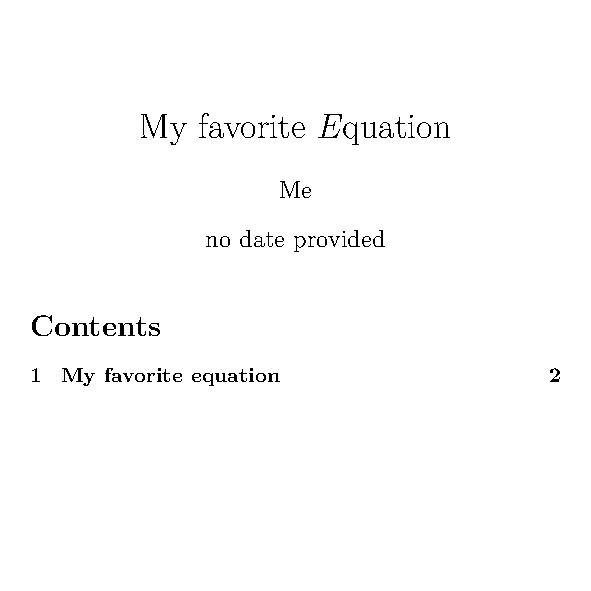
\includegraphics[height=0.7\textheight, page=1]{exStrutLvl1}}
        \end{column}
        \begin{column}{0.5\textwidth}
            \fbox{\includegraphics[height=0.7\textheight, page=2]{exStrutLvl1}}
        \end{column}
    \end{columns}
    
\end{frame}

\begin{frame}{\exFrame{Try to reproduce the following}}{lvl 2. The 2025 year must be ``current year'', not just ``2025''! \textit{You may need to google some stuff}}\relax
    
    \begin{columns}
        \begin{column}{0.5\textwidth}
            \fbox{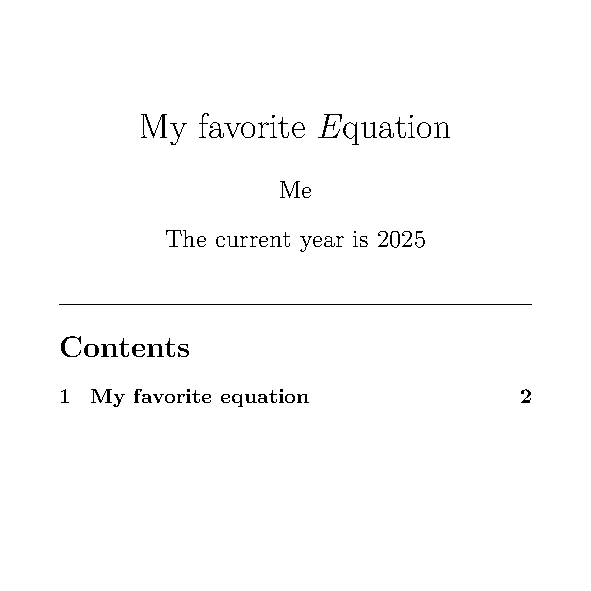
\includegraphics[height=0.7\textheight, page=1]{exStrutLvl2}}
        \end{column}
        \begin{column}{0.5\textwidth}
            \fbox{\includegraphics[height=0.7\textheight, page=2]{exStrutLvl2}}
        \end{column}
    \end{columns}
\end{frame}
}


\subsection{References}
% \knuthc  knuth the TeXBook
% \lvoc   Lvovsky
% \lamc  lamport latex 
% \slshape different font for footnote
\graphicspath{{sec01/images/s2/}{sec01/code/s2/}}
\lstset{inputpath=sec01/code/s2/}

\begin{frame}[fragile]{How good it will be if...\only<2,3>{we could write like this}}\relax
\begin{center}
\only<1>{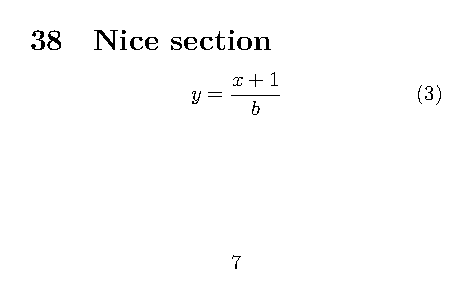
\includegraphics{refBegin}}
\only<2>{\includegraphics{refBegin2}}
\only<3>{\Huge We can!}
\end{center}

\cprotect\skfootnote{I use \verb|\only<2>{text}| for such effect. Also \verb|\setcounter| was used in source.}
\end{frame}

\begin{frame}[fragile]{Step 1: \ccol\label}\relax
    %  \lstinputlisting[linerange={12-15}]{refBegin2.tex}
     \inputminted[firstline=12, lastline=15, fontsize=\tt]{latex}{sec01/code/s2/refBegin2.tex}
     
     \skfootnote{for whole reference mechanism: \lmanc{7}[51] \lvoc{I.2.11}[27] \overC{https://www.overleaf.com/learn/latex/Cross_referencing_sections_and_equations}, \wikiC{https://en.wikibooks.org/wiki/LaTeX/Labels_and_Cross-referencing}}
\end{frame}

\begin{frame}[fragile]{Step 2: \ccol{\ref} and \ccol{\pageref}}
%, basicstyle=\tt
    %  \lstinputlisting[linerange={17-17}]{refBegin2.tex}
     \inputminted[firstline=17, lastline=17, fontsize=\tt]{latex}{sec01/code/s2/refBegin2.tex}
\end{frame}

\begin{frame}[fragile]{Combined}\relax
     \inputminted[firstline=12, lastline=17, fontsize=\tt]{latex}{sec01/code/s2/refBegin2.tex}
     
\inpause Notice \texttt{prefix\ccol{:}id} notation (\texttt{sec:nice}). It is rather common

\end{frame}

\begin{frame}[fragile]{Problem 1: lots of labels!}
    What if you have too many marks throughout the document?
    \inclasshigh{\inpause Will you have to open the .tex on the left, the .pdf on the right and compare them line by line? }
    \inpause
    
    Use package \ccol{showlabels}
\cprotect\twocolImg{
% , basicstyle=\tt\smal
    % \lstinputlisting[linerange={10-10, 13-16}]{refBeginShow.tex}
    \inputminted[firstline=10, lastline=10]{latex}{sec01/code/s2/refBeginShow.tex}
    \inputminted[firstline= 13, lastline=16]{latex}{sec01/code/s2/refBeginShow.tex}
}{refBeginShow}    
    
    
    \skfootnote{\url{http://ctan.altspu.ru/macros/latex/contrib/showlabels/showlabels.pdf}}
\end{frame}

\begin{frame}[fragile]{Problem 2: Typos}\relax
\cprotect\twocolImg{
% , basicstyle=\tt\small
    % \lstinputlisting[linerange={12-17}]{refBad.tex}
    \inputminted[firstline=12, lastline=17]{latex}{sec01/code/s2/refBad.tex}
}{refBad}

\inpause
Look at \textbf{?} in the document or inside the logs
\end{frame}

\begin{frame}[fragile]{Counter domination}\relax

look at the equation numbering style
\cprotect\twocolImg{
    \inputminted[firstline=11, lastline=19]{latex}{sec01/code/s2/refDomination.tex}
}{refDomination}

\end{frame}

\begin{frame}[fragile]{Bibliography}{How to cite}\relax
Use \ccol{\cite\{label\}}

\cprotect\twocolImg{
% , basicstyle=\tt\small
    % \lstinputlisting[linerange={9-9}]{citeFirst.tex}
    \inputminted[firstline=9, lastline=9, fontsize=\tt]{latex}{sec01/code/s2/citeFirst.tex}
}{citeFirst}  

\inpause
\cprotect\twocolImg{
% , basicstyle=\tt\small
    % \lstinputlisting[linerange={11-12}]{citeSecond.tex}
    \inputminted[firstline=11, lastline=12, fontsize=\tt]{latex}{sec01/code/s2/citeSecond.tex}
}{citeSecond}  

\skfootnote{\lmanc{8.24.2}[94] \wikiC{https://en.wikibooks.org/wiki/LaTeX/Bibliography_Management} \overC{https://www.overleaf.com/learn/latex/Bibliography_management_in_LaTeX}}     
\end{frame}

\begin{frame}[fragile]{Bibliography}{What to cite}\relax

{\csk .bib} files

\begin{verbatim}
@Book{landau,
    author = {Landau, L. D. and Lifshitz, E. M.},
    title = {The Classical Theory of Fields},
    journal = N,
    volume = {1},
    pages = {140},
    year = 1980
}
\end{verbatim}

You can have multiple records in one .bib file.
     
\end{frame}

\begin{frame}[fragile]{Offline - compile twice!}\relax
Running \LaTeX\ offline, you can get \textbf{(??)} in \ccol{\ref} and \textbf{[?]} in \ccol{\cite}. 

For 
\begin{itemize}
    \item References 
    \item Bibliography
    \item Table of content
    \item Indexing
    \item ...
\end{itemize}

\LaTeX\ collect addition data in extra files. \LaTeX\ need more then one run to get this data. 

Use \verb|latex; bibtex; latex; latex|

\inclasshigh{we will talk about the mechanism in the last lecture}

\end{frame}

\begin{frame}[fragile]{Bibliography. Where can you get .bib files?}\relax
\begin{itemize}
    \item Just google it! ``article\_name bibtex''
    \item at \url{scholar.google.ru} ask Cite -> BibTeX
    \item Go to your favorite journal and look at Citations -> ``.bib'' or ``bibtex''
    \item Ask Mendeley, Zotero or other programs to give you the .bib file
    \item Create it by yourself
\end{itemize}
\end{frame}

\begin{frame}[fragile]{Bibliography. Creating .bib file \magicPage}\relax
\begin{center}
\begin{tabular}{rl}
     \ccol{@article} & Journal or magazine article\\
\ccol{@book} & Book\\
\ccol{@conference} & Article in conference proceedings\\
\ccol{@misc} & If nothing else fits.
\end{tabular}
\end{center}

Than fill in 

{\obeylines 
\ author
\ title
\ journal
\ year
\ pages
\ volume}

following the example of other entries

\skfootnote{\wikiC{https://en.wikibooks.org/wiki/LaTeX/Bibliography_Management\#Standard_templates} for cite url checkout \stExC{https://tex.stackexchange.com/questions/3587/how-can-i-use-bibtex-to-cite-a-web-page}\\ check for full list \wikiC{https://en.wikibooks.org/wiki/LaTeX/Bibliography_Management\#BibTeX}
}     
\end{frame}

% \newcommand{\twocolImgS}[2]{  % add two columns: (1) is some text (2) is an image.
%     \begin{columns}
%         \begin{column}{0.45\textwidth}
%             #1
%         \end{column}
%         \begin{column}{0.45\textwidth}
%         \fbox{\includegraphics[width=\textwidth, keepaspectratio,page=1]{#2}}
        
%         \fbox{\includegraphics[width=\textwidth, keepaspectratio,page=2]{#2}}
%         % ниже мы делаем позиционирование, поднимая изображение на половину его высоты. Таким образом, центрированные слайды останутся центрированными и с т.з. изображения
%             % https://tex.stackexchange.com/questions/3166/how-can-the-dimensions-of-a-box-be-retrieved-with-latex
%             % \savebox{\Abox}{\includegraphics[width=\textwidth, keepaspectratio,page=1]{#2}\\\hrule\includegraphics[width=\textwidth, keepaspectratio,page=2]{#2}}
%             % \newlength{\myhh}
%             % \settoheight{\myhh}{\usebox{\Abox}}
%             % \raisebox{-0.5\myhh+1ex}[0pt][0pt]{\includegraphics[width=\textwidth, keepaspectratio,page=1]{#2}\\\hrule\includegraphics[width=\textwidth, keepaspectratio,page=2]{#2}}
%         \end{column}
%     \end{columns}
% }

% \begin{frame}[fragile]{Bibliography. Manually\magicPage}

% You can add Bibliography manually.

% \cprotect\twocolImg{
%     \inputminted[firstline=10, lastline=22]{latex}{sec01/code/s2/citeMan.tex}
%     % \lstinputlisting[linerange={10-22}]{citeMan.tex}
% }{citeMan}  

% \skfootnote{\lmanc{8.24}[92]}
% \end{frame}

% \begin{frame}[fragile]{Bibliography. Styles\magicPage}

% You can change styles.

% Mannually -- check \url{https://en.wikibooks.org/wiki/LaTeX/Bibliography_Management}

% Or with packages -- check \url{https://tex.stackexchange.com/questions/25701/bibtex-vs-biber-and-biblatex-vs-natbib}
% \end{frame}

% \begin{frame}[fragile]{Nomenclature\magicPage}\relax

%     \cprotect\twocolImg{
%         % \inputminted[firstline=9, lastline=16]{latex}{sec01/code/s2/indexmy.tex}
%         \inputminted[firstline=8, lastline=14]{latex}{sec01/code/s2/nomenclature.tex}
%     }{nomenclature}  

%     \skfootnote{\overC{https://www.overleaf.com/learn/latex/Nomenclatures}}     
% \end{frame}

% \begin{frame}[fragile]{Subject index\magicPage}\relax % предметный указатель

% \cprotect\twocolImgS{
%     \inputminted[firstline=9, lastline=16]{latex}{sec01/code/s2/indexmy.tex}
% }{indexmy}


% \skfootnote{\lvoc{IV.7}[175] \lmanc{25.2}[215]}     
% \end{frame}



\subsection{Useful commands}
% \knuthc  knuth the TeXBook
% \lvoc   Lvovsky
% \lamc  lamport latex 
% \slshape different font for footnote
\graphicspath{{sec01/images/s3/}{sec01/code/s3/}}
\lstset{inputpath=sec01/code/s3/}

\begin{frame}[fragile]{\ccol{\footnote}\magicPage}\relax
\cprotect\twocolImg{
    % \lstinputlisting[linerange={9-9}]{footnoteMy.tex}
    \inputminted[firstline=9, lastline=9]{latex}{sec01/code/s3/footnoteMy.tex}
}{footnoteMy}  


\skfootnote{\lmanc{8}[108] \wikiC{https://en.wikibooks.org/wiki/LaTeX/Footnotes_and_Margin_Notes} \overC{https://www.overleaf.com/learn/latex/Footnotes} \knuthc{15}[120]}
\end{frame}

\begin{frame}[fragile]{Horizontal aligment\magicPage}\relax
\cprotect\twocolImg{
    % \lstinputlisting[linerange={9-25}]{flushing.tex}
    \inputminted[firstline=9, lastline=25]{latex}{sec01/code/s3/flushing.tex}
}{flushing}  


\skfootnote{\lmanc{8.12}[63] \lmanc{8.13}[64] \knuthc{14}[112] and note \stExC{https://tex.stackexchange.com/questions/64644/centering-doesnt-seem-to-center-my-text}}
\end{frame}

\begin{frame}[fragile]{Page break\magicPage}\relax

{\centering \Large \ccol{\newpage} \ccol{\pagebreak}\par}

\skfootnote{\lmanc{10}[105] \stExC{https://tex.stackexchange.com/questions/736/pagebreak-vs-newpage}}
     
\end{frame}

\begin{frame}[fragile]{Quotes\magicPage}\relax

\cprotect\twocolImg{
    % \lstinputlisting[linerange={10-14}]{quotemy.tex}
    \inputminted[firstline=10, lastline=14]{latex}{sec01/code/s3/quotemy.tex}
}{quotemy}  


\cprotect\skfootnote{\lvoc{III.7.1}[129] \lmanc{8.20}[83]. Also see \verb|quotation| env }
     
\end{frame}

\begin{frame}[fragile]{Verses\magicPage}\relax

\cprotect\twocolImg{
    % \lstinputlisting[linerange={11-18}]{versemy.tex}
    \inputminted[firstline=11, lastline=18]{latex}{sec01/code/s3/versemy.tex}
}{versemy}  

\skfootnote{\lvoc{III.7.3}[130] \lmanc{8.28}[98]}
\end{frame}

\begin{frame}[fragile]{Marginal notes\magicPage}\relax

\cprotect\twocolImg{
    % \lstinputlisting[linerange={9-10}]{marginmy.tex}
    \inputminted[firstline=9, lastline=10]{latex}{sec01/code/s3/marginmy.tex}
}{marginmy}  

\skfootnote{\lvoc{IV.10}[194] \lmanc{15.4}[137]}
\end{frame}

 
 %%%%%%%%%% in class tasks %%%%%%%%%%%%%%%%%
 
 \cprotect\inclassframe{
 \begin{frame}{\exFrame{Create a document}}{lvl 1}\relax
 ...with following params
 
 \begin{itemize}
     \item it must be an article
     \item it must contains at least two pages 
     \item it must have an equation 
     \item it must refer to the equation number
      
 \end{itemize}
      
 \end{frame}
 
 \begin{frame}{\exFrame{Create a document}}{lvl 2}\relax
 ...with following params
 
 \begin{itemize}
     \item it must be an article
     \item it must contains at least two pages 
     \item it must have an equation 
     \item it must refer to the equation number
     \item it must contains a theorem (google for it)
     \item it must have at least two sections and subsections
     \item the equation numbering must be (section.subsection.equation) 
      
 \end{itemize}
      
 \end{frame}
 
 }
% \cprotect\inclassFrame{
% \begin{frame}[fragile]{Try to add a package}\relax
% \url{http://hanno-rein.de/downloads/coffee.sty}

% and use \verb|\newpage \coffee{2} hello world!|

% \inpause
% NOW you document is ready!

% \end{frame}
% }


%% It is just an empty TeX file.
%% Write your code here.
\graphicspath{{sec01/images/}{sec01/code/}}
\lstset{inputpath=sec01/code/}


\begin{frame}{How to structure \& refer the document}\relax
    \begin{center}
        \includegraphics{s2/refBegin2}
    \end{center}
    
\end{frame}

\begin{frame}{How to structure \& refer the document}\relax
    \begin{enumerate}
         $\left.
         \begin{tabular}{p{.5\textwidth}} \vspace{-2ex}
         \item add structure element. \TeX\ will automatically calculate it's serial number incrementing the previous one. 
         \item refer to the element added before or after label. Refer to specific page, to specific equation, to specific biblio record or item
         \end{tabular}
         \right\}\text{\TeX\ use ``counters'' implicitly}$
     \end{enumerate}     
\end{frame}

% общая идея: счётчики, подчинение счётчиков, двойной прогон
\begin{frame}{how all this works}\relax
% отдельно счётчики
% отдельно labels
% и слайд что это отдельно 
\begin{enumerate}
    \item \TeX\ has a counter for... lots of stuff 
    \item When you add an element (section, equation, etc), the command updates its counter and prints it near the element\inpause
    \item To reference an element, you need to explicitly tell \TeX\ about it.
    \item When \TeX\ ``sees'' this guideline, it saves the related counter to {\csk external} file
    \item When \TeX\ runs {\csk second time} and finds the place where you need to insert the reference, it looks at the file and gets counter value from the file \inpause
    \item Sometimes (e.g.: bibliography) you run external command (e.g.: bibtex) to create the mentioned file \inpause
    \item By the way: \TeX\ always ``reads'' document from top to bottom. \outclasshigh{The only way some command to affect anything \textit{before} the command appears is throw external file. The set of commands that do this is quite small}
\end{enumerate}

\inpause 
(We will look more precisely at the last lecture.)
     
\end{frame}

\subsection{Structural elements}
% \knuthc  knuth the TeXBook
% \lvoc   Lvovsky
% \lamc  lamport latex 
% \slshape different font for footnote
\graphicspath{{sec01/images/s1z/}{sec01/code/s1/}}
\lstset{inputpath=sec01/code/s1/}

\begin{frame}{What document consists of?}\relax
\begin{itemize}
    \item Title
    \item Authors
    \item Table of contents
    \item Table of figures
    \item Table of tables
    \item Sections, subsections,..
    % \item Bibliography
\end{itemize}
     
\end{frame}

%%%%%%%%%%%%%%%%%%%% Title %%%%%%%%%%%%%%%%%%%%%%
\begin{frame}[fragile]{Title}{title}\relax
\cprotect\twocolImg{
% \lstinputlisting[linerange={6-9}]{title01.tex}
\inputminted[firstline=6, lastline=9]{latex}{sec01/code/s1/title01.tex}
}{title01}
\inpause
\begin{itemize}
     \item \ccol{\title} before begin of the document
     \item \ccol{\maketitle} after begin of the document 
\end{itemize}
% \inclassFrag{Try it in your own paper!}[-1]
\skfootnote{\wikiC{https://en.wikibooks.org/wiki/LaTeX/Title_Creation} \lmanc{18.1}[163] \lmanc{8.26}[96]}
\end{frame}

\begin{frame}[fragile]{Title}{date}
 \cprotect\twocolImg{
% \lstinputlisting[linerange={6-10}]{title02.tex}
\inputminted[firstline=6, lastline=10]{latex}{sec01/code/s1/title02.tex}
}{title02}
\inpause
\begin{itemize}
     \item by defaut \LaTeX\ think you use {\csk \verb|\date{\today}|}
     \inclassFrag{what do you think command \ccol{\today} if for?}[3]
     \begin{itemize}
         \item \ccol{\today} is the date of last document compilation
     \end{itemize} 
     \inpause
     \item you can put anything inside \ccol{\date}\{\} command
     \item use \ccol{\date}\{\} without arguments to remove the string
\end{itemize}
\inpause
\inclasshigh{notice \ccol\the\ before year, month and day. We will return to it at the last lecture}
\end{frame}

\begin{frame}[fragile]{Title}{authors}
 \cprotect\twocolImg{
% \lstinputlisting[linerange={6-11}]{title03.tex}
\inputminted[firstline=6, lastline=11]{latex}{sec01/code/s1/title03.tex}
}{title03}

\inpause
\begin{itemize}
    \item \ccol\author\ for put the author
    \item \ccol\and\ (can be) used to concatinate several authors
    \begin{itemize}
        \item You always can use just plain text
    \end{itemize}
    \item \ccol\thanks\ for a footnote 
\end{itemize}
\end{frame}

\begin{frame}[fragile]{Abstract}\relax
\cprotect\twocolImg{
    \inputminted[firstline=8, lastline=10]{latex}{sec01/code/s1/abstractmy.tex}
    % \lstinputlisting[linerange={8-10}]{abstractmy.tex}
}{abstractmy}

% \inpause\inclasshigh{...Nothing happends, yeah?))}

% \outclasshigh{The style of abstract may change in specific journal, but by default there is no addition style}

\skfootnote{\lmanc{8.1}[54] \lvoc{IV.5.4}[170]}
\end{frame}

\begin{frame}[fragile]{Structure}\relax
\cprotect\twocolImg{
    \inputminted[firstline=7, lastline=15]{latex}{sec01/code/s1/struc.tex}
    % \lstinputlisting[linerange={7-15}]{struc.tex}
}{struc}

    \cprotect\skfootnote{\wikiC{https://en.wikibooks.org/wiki/LaTeX/Document_Structure\#Section_numbering}, \overC{https://www.overleaf.com/learn/latex/Sections_and_chapters}, \lmanc{6}[40], \lvoc{IV.5}[165]\\ 
    You can use \verb|\section[short name]{long name}| to put \verb|short name| to table of contents and \verb|\renewcommand{\chaptername}{new name}| (\lvoc{IV.5.3}[169]) to change the standard name
    }
\end{frame}


\begin{frame}[fragile]{Structure}{Tips}\relax

% \inclassFrag{Try \ccol\section*}[1]

\begin{itemize}
    \item Use {\csk \textbackslash<command>*} (with {\Large *}) to ommit the numbering
    \item The structure (and titles) is not pre-build into \LaTeX: they are defined inside class files $\Rightarrow$ not all classes contain all commands
     
\end{itemize}
\end{frame}

\begin{frame}[fragile]{Table of content}\relax
\cprotect\twocolImg{
    \inputminted[firstline=8, lastline=16]{latex}{sec01/code/s1/toc.tex}
    % \lstinputlisting[linerange={8-16}]{toc.tex}
}{toc}
     \inpause \ccol{\tableofcontents} for create it, \ccol{\newpage} for new page.
     
     Notice that not all structure elements are mentioned it ToC!

     \cprotect\skfootnote{\lmanc{25.1}[212]\\
     \verb|\contentsname| --- the name of the ToC; \verb|secnumdepth| counter (\lvoc{IX.3.1}[298], \lmanc{6}[40]) to change what will be included in ToC
     }
\end{frame}



\begin{frame}[fragile]{Table of...}\relax
\Large
     \begin{itemize}
          \item \ccol{\listoffigures} for figures 
          \item \ccol{\listoftables} for tables 
     \end{itemize}
     
     \cprotect\skfootnote{\lvoc{IV.8.1}[188], \lmanc{25.1}[202]\\ 
     You can use \verb|\caption[short name]{long name}| to put \verb|short name| to the lists, \verb|\listfigurename| and \verb|\listtablename| --- the names of the Lists.
     }
\end{frame}

%%%%%%%%%%%%%% IN CLASS EXERSISES
% different classes
\cprotect\inclassframe{
\begin{frame}[fragile]{\exFrame{Try to use the commands for different class files}}\relax
    \inputminted{latex}{sec01/code/s1/strucTask.tex}
    %  \lstinputlisting[linerange={1-1,7-15},basicstyle=\tt\small]{strucTask.tex}
    %  
     for {\csk book, report, article}
     
\end{frame}
}

\inclassframe{
\begin{frame}{\exFrame{Try to reproduce the following}}{lvl 1}\relax
    \begin{columns}
        \begin{column}{0.5\textwidth}
            \fbox{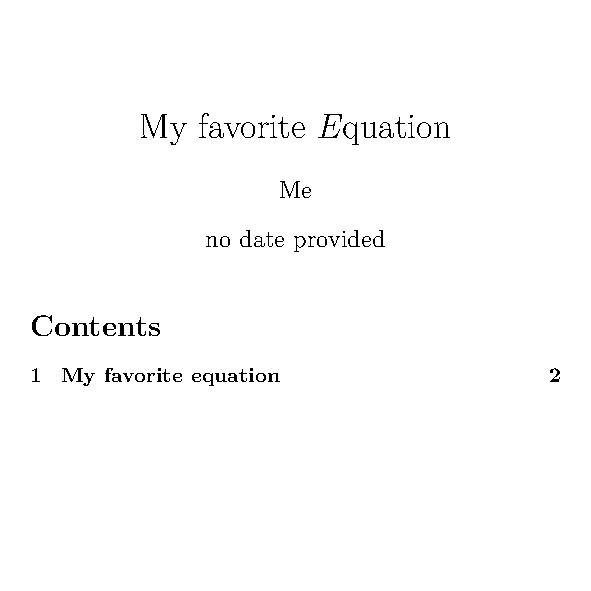
\includegraphics[height=0.7\textheight, page=1]{exStrutLvl1}}
        \end{column}
        \begin{column}{0.5\textwidth}
            \fbox{\includegraphics[height=0.7\textheight, page=2]{exStrutLvl1}}
        \end{column}
    \end{columns}
    
\end{frame}

\begin{frame}{\exFrame{Try to reproduce the following}}{lvl 2. The 2025 year must be ``current year'', not just ``2025''! \textit{You may need to google some stuff}}\relax
    
    \begin{columns}
        \begin{column}{0.5\textwidth}
            \fbox{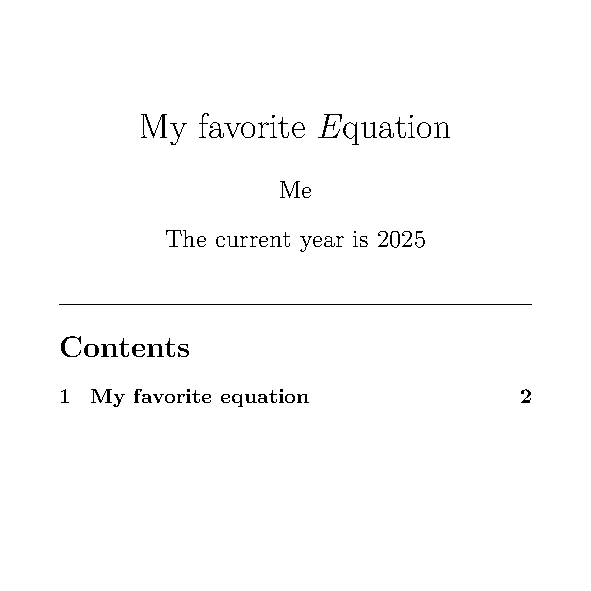
\includegraphics[height=0.7\textheight, page=1]{exStrutLvl2}}
        \end{column}
        \begin{column}{0.5\textwidth}
            \fbox{\includegraphics[height=0.7\textheight, page=2]{exStrutLvl2}}
        \end{column}
    \end{columns}
\end{frame}
}


\subsection{References}
% \knuthc  knuth the TeXBook
% \lvoc   Lvovsky
% \lamc  lamport latex 
% \slshape different font for footnote
\graphicspath{{sec01/images/s2/}{sec01/code/s2/}}
\lstset{inputpath=sec01/code/s2/}

\begin{frame}[fragile]{How good it will be if...\only<2,3>{we could write like this}}\relax
\begin{center}
\only<1>{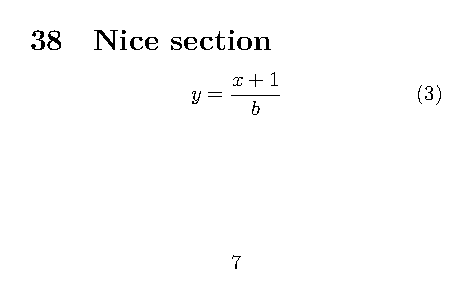
\includegraphics{refBegin}}
\only<2>{\includegraphics{refBegin2}}
\only<3>{\Huge We can!}
\end{center}

\cprotect\skfootnote{I use \verb|\only<2>{text}| for such effect. Also \verb|\setcounter| was used in source.}
\end{frame}

\begin{frame}[fragile]{Step 1: \ccol\label}\relax
    %  \lstinputlisting[linerange={12-15}]{refBegin2.tex}
     \inputminted[firstline=12, lastline=15, fontsize=\tt]{latex}{sec01/code/s2/refBegin2.tex}
     
     \skfootnote{for whole reference mechanism: \lmanc{7}[51] \lvoc{I.2.11}[27] \overC{https://www.overleaf.com/learn/latex/Cross_referencing_sections_and_equations}, \wikiC{https://en.wikibooks.org/wiki/LaTeX/Labels_and_Cross-referencing}}
\end{frame}

\begin{frame}[fragile]{Step 2: \ccol{\ref} and \ccol{\pageref}}
%, basicstyle=\tt
    %  \lstinputlisting[linerange={17-17}]{refBegin2.tex}
     \inputminted[firstline=17, lastline=17, fontsize=\tt]{latex}{sec01/code/s2/refBegin2.tex}
\end{frame}

\begin{frame}[fragile]{Combined}\relax
     \inputminted[firstline=12, lastline=17, fontsize=\tt]{latex}{sec01/code/s2/refBegin2.tex}
     
\inpause Notice \texttt{prefix\ccol{:}id} notation (\texttt{sec:nice}). It is rather common

\end{frame}

\begin{frame}[fragile]{Problem 1: lots of labels!}
    What if you have too many marks throughout the document?
    \inclasshigh{\inpause Will you have to open the .tex on the left, the .pdf on the right and compare them line by line? }
    \inpause
    
    Use package \ccol{showlabels}
\cprotect\twocolImg{
% , basicstyle=\tt\smal
    % \lstinputlisting[linerange={10-10, 13-16}]{refBeginShow.tex}
    \inputminted[firstline=10, lastline=10]{latex}{sec01/code/s2/refBeginShow.tex}
    \inputminted[firstline= 13, lastline=16]{latex}{sec01/code/s2/refBeginShow.tex}
}{refBeginShow}    
    
    
    \skfootnote{\url{http://ctan.altspu.ru/macros/latex/contrib/showlabels/showlabels.pdf}}
\end{frame}

\begin{frame}[fragile]{Problem 2: Typos}\relax
\cprotect\twocolImg{
% , basicstyle=\tt\small
    % \lstinputlisting[linerange={12-17}]{refBad.tex}
    \inputminted[firstline=12, lastline=17]{latex}{sec01/code/s2/refBad.tex}
}{refBad}

\inpause
Look at \textbf{?} in the document or inside the logs
\end{frame}

\begin{frame}[fragile]{Counter domination}\relax

look at the equation numbering style
\cprotect\twocolImg{
    \inputminted[firstline=11, lastline=19]{latex}{sec01/code/s2/refDomination.tex}
}{refDomination}

\end{frame}

\begin{frame}[fragile]{Bibliography}{How to cite}\relax
Use \ccol{\cite\{label\}}

\cprotect\twocolImg{
% , basicstyle=\tt\small
    % \lstinputlisting[linerange={9-9}]{citeFirst.tex}
    \inputminted[firstline=9, lastline=9, fontsize=\tt]{latex}{sec01/code/s2/citeFirst.tex}
}{citeFirst}  

\inpause
\cprotect\twocolImg{
% , basicstyle=\tt\small
    % \lstinputlisting[linerange={11-12}]{citeSecond.tex}
    \inputminted[firstline=11, lastline=12, fontsize=\tt]{latex}{sec01/code/s2/citeSecond.tex}
}{citeSecond}  

\skfootnote{\lmanc{8.24.2}[94] \wikiC{https://en.wikibooks.org/wiki/LaTeX/Bibliography_Management} \overC{https://www.overleaf.com/learn/latex/Bibliography_management_in_LaTeX}}     
\end{frame}

\begin{frame}[fragile]{Bibliography}{What to cite}\relax

{\csk .bib} files

\begin{verbatim}
@Book{landau,
    author = {Landau, L. D. and Lifshitz, E. M.},
    title = {The Classical Theory of Fields},
    journal = N,
    volume = {1},
    pages = {140},
    year = 1980
}
\end{verbatim}

You can have multiple records in one .bib file.
     
\end{frame}

\begin{frame}[fragile]{Offline - compile twice!}\relax
Running \LaTeX\ offline, you can get \textbf{(??)} in \ccol{\ref} and \textbf{[?]} in \ccol{\cite}. 

For 
\begin{itemize}
    \item References 
    \item Bibliography
    \item Table of content
    \item Indexing
    \item ...
\end{itemize}

\LaTeX\ collect addition data in extra files. \LaTeX\ need more then one run to get this data. 

Use \verb|latex; bibtex; latex; latex|

\inclasshigh{we will talk about the mechanism in the last lecture}

\end{frame}

\begin{frame}[fragile]{Bibliography. Where can you get .bib files?}\relax
\begin{itemize}
    \item Just google it! ``article\_name bibtex''
    \item at \url{scholar.google.ru} ask Cite -> BibTeX
    \item Go to your favorite journal and look at Citations -> ``.bib'' or ``bibtex''
    \item Ask Mendeley, Zotero or other programs to give you the .bib file
    \item Create it by yourself
\end{itemize}
\end{frame}

\begin{frame}[fragile]{Bibliography. Creating .bib file \magicPage}\relax
\begin{center}
\begin{tabular}{rl}
     \ccol{@article} & Journal or magazine article\\
\ccol{@book} & Book\\
\ccol{@conference} & Article in conference proceedings\\
\ccol{@misc} & If nothing else fits.
\end{tabular}
\end{center}

Than fill in 

{\obeylines 
\ author
\ title
\ journal
\ year
\ pages
\ volume}

following the example of other entries

\skfootnote{\wikiC{https://en.wikibooks.org/wiki/LaTeX/Bibliography_Management\#Standard_templates} for cite url checkout \stExC{https://tex.stackexchange.com/questions/3587/how-can-i-use-bibtex-to-cite-a-web-page}\\ check for full list \wikiC{https://en.wikibooks.org/wiki/LaTeX/Bibliography_Management\#BibTeX}
}     
\end{frame}

% \newcommand{\twocolImgS}[2]{  % add two columns: (1) is some text (2) is an image.
%     \begin{columns}
%         \begin{column}{0.45\textwidth}
%             #1
%         \end{column}
%         \begin{column}{0.45\textwidth}
%         \fbox{\includegraphics[width=\textwidth, keepaspectratio,page=1]{#2}}
        
%         \fbox{\includegraphics[width=\textwidth, keepaspectratio,page=2]{#2}}
%         % ниже мы делаем позиционирование, поднимая изображение на половину его высоты. Таким образом, центрированные слайды останутся центрированными и с т.з. изображения
%             % https://tex.stackexchange.com/questions/3166/how-can-the-dimensions-of-a-box-be-retrieved-with-latex
%             % \savebox{\Abox}{\includegraphics[width=\textwidth, keepaspectratio,page=1]{#2}\\\hrule\includegraphics[width=\textwidth, keepaspectratio,page=2]{#2}}
%             % \newlength{\myhh}
%             % \settoheight{\myhh}{\usebox{\Abox}}
%             % \raisebox{-0.5\myhh+1ex}[0pt][0pt]{\includegraphics[width=\textwidth, keepaspectratio,page=1]{#2}\\\hrule\includegraphics[width=\textwidth, keepaspectratio,page=2]{#2}}
%         \end{column}
%     \end{columns}
% }

% \begin{frame}[fragile]{Bibliography. Manually\magicPage}

% You can add Bibliography manually.

% \cprotect\twocolImg{
%     \inputminted[firstline=10, lastline=22]{latex}{sec01/code/s2/citeMan.tex}
%     % \lstinputlisting[linerange={10-22}]{citeMan.tex}
% }{citeMan}  

% \skfootnote{\lmanc{8.24}[92]}
% \end{frame}

% \begin{frame}[fragile]{Bibliography. Styles\magicPage}

% You can change styles.

% Mannually -- check \url{https://en.wikibooks.org/wiki/LaTeX/Bibliography_Management}

% Or with packages -- check \url{https://tex.stackexchange.com/questions/25701/bibtex-vs-biber-and-biblatex-vs-natbib}
% \end{frame}

% \begin{frame}[fragile]{Nomenclature\magicPage}\relax

%     \cprotect\twocolImg{
%         % \inputminted[firstline=9, lastline=16]{latex}{sec01/code/s2/indexmy.tex}
%         \inputminted[firstline=8, lastline=14]{latex}{sec01/code/s2/nomenclature.tex}
%     }{nomenclature}  

%     \skfootnote{\overC{https://www.overleaf.com/learn/latex/Nomenclatures}}     
% \end{frame}

% \begin{frame}[fragile]{Subject index\magicPage}\relax % предметный указатель

% \cprotect\twocolImgS{
%     \inputminted[firstline=9, lastline=16]{latex}{sec01/code/s2/indexmy.tex}
% }{indexmy}


% \skfootnote{\lvoc{IV.7}[175] \lmanc{25.2}[215]}     
% \end{frame}



\subsection{Useful commands}
% \knuthc  knuth the TeXBook
% \lvoc   Lvovsky
% \lamc  lamport latex 
% \slshape different font for footnote
\graphicspath{{sec01/images/s3/}{sec01/code/s3/}}
\lstset{inputpath=sec01/code/s3/}

\begin{frame}[fragile]{\ccol{\footnote}\magicPage}\relax
\cprotect\twocolImg{
    % \lstinputlisting[linerange={9-9}]{footnoteMy.tex}
    \inputminted[firstline=9, lastline=9]{latex}{sec01/code/s3/footnoteMy.tex}
}{footnoteMy}  


\skfootnote{\lmanc{8}[108] \wikiC{https://en.wikibooks.org/wiki/LaTeX/Footnotes_and_Margin_Notes} \overC{https://www.overleaf.com/learn/latex/Footnotes} \knuthc{15}[120]}
\end{frame}

\begin{frame}[fragile]{Horizontal aligment\magicPage}\relax
\cprotect\twocolImg{
    % \lstinputlisting[linerange={9-25}]{flushing.tex}
    \inputminted[firstline=9, lastline=25]{latex}{sec01/code/s3/flushing.tex}
}{flushing}  


\skfootnote{\lmanc{8.12}[63] \lmanc{8.13}[64] \knuthc{14}[112] and note \stExC{https://tex.stackexchange.com/questions/64644/centering-doesnt-seem-to-center-my-text}}
\end{frame}

\begin{frame}[fragile]{Page break\magicPage}\relax

{\centering \Large \ccol{\newpage} \ccol{\pagebreak}\par}

\skfootnote{\lmanc{10}[105] \stExC{https://tex.stackexchange.com/questions/736/pagebreak-vs-newpage}}
     
\end{frame}

\begin{frame}[fragile]{Quotes\magicPage}\relax

\cprotect\twocolImg{
    % \lstinputlisting[linerange={10-14}]{quotemy.tex}
    \inputminted[firstline=10, lastline=14]{latex}{sec01/code/s3/quotemy.tex}
}{quotemy}  


\cprotect\skfootnote{\lvoc{III.7.1}[129] \lmanc{8.20}[83]. Also see \verb|quotation| env }
     
\end{frame}

\begin{frame}[fragile]{Verses\magicPage}\relax

\cprotect\twocolImg{
    % \lstinputlisting[linerange={11-18}]{versemy.tex}
    \inputminted[firstline=11, lastline=18]{latex}{sec01/code/s3/versemy.tex}
}{versemy}  

\skfootnote{\lvoc{III.7.3}[130] \lmanc{8.28}[98]}
\end{frame}

\begin{frame}[fragile]{Marginal notes\magicPage}\relax

\cprotect\twocolImg{
    % \lstinputlisting[linerange={9-10}]{marginmy.tex}
    \inputminted[firstline=9, lastline=10]{latex}{sec01/code/s3/marginmy.tex}
}{marginmy}  

\skfootnote{\lvoc{IV.10}[194] \lmanc{15.4}[137]}
\end{frame}

 
 %%%%%%%%%% in class tasks %%%%%%%%%%%%%%%%%
 
 \cprotect\inclassframe{
 \begin{frame}{\exFrame{Create a document}}{lvl 1}\relax
 ...with following params
 
 \begin{itemize}
     \item it must be an article
     \item it must contains at least two pages 
     \item it must have an equation 
     \item it must refer to the equation number
      
 \end{itemize}
      
 \end{frame}
 
 \begin{frame}{\exFrame{Create a document}}{lvl 2}\relax
 ...with following params
 
 \begin{itemize}
     \item it must be an article
     \item it must contains at least two pages 
     \item it must have an equation 
     \item it must refer to the equation number
     \item it must contains a theorem (google for it)
     \item it must have at least two sections and subsections
     \item the equation numbering must be (section.subsection.equation) 
      
 \end{itemize}
      
 \end{frame}
 
 }
% \cprotect\inclassFrame{
% \begin{frame}[fragile]{Try to add a package}\relax
% \url{http://hanno-rein.de/downloads/coffee.sty}

% and use \verb|\newpage \coffee{2} hello world!|

% \inpause
% NOW you document is ready!

% \end{frame}
% }

\graphicspath{{sec/images/}{sec/code/}}
\lstset{inputpath=sec/code/}

\section{\TeX\ primitives}

\begin{frame}{Entities}

    \begin{enumerate}
        \item Primitive commands
        \item Counters (=integer numbers)
        \item Lengths
        \item Boxes
        \item Glues
        \item Spaces 
        \item Toks (Strings)
        \item Inserts 
    \end{enumerate}
    \inpause
    commands and macros will wait in details the next lecture. No we discuss it just in a few words
\end{frame}

\subsection{Commands (Macros)}


\begin{frame}[fragile]{Simple command creation \lW}\relax
    \twocolImg{
    \inputminted[firstline=8, lastline=8]{latex}{sec/code/commandSimple.tex}
    \inputminted[firstline=13, lastline=20]{latex}{sec/code/commandSimple.tex}
    }{commandSimple}
    
    \inpause
    \inclasshigh{You are a developer now!}
\end{frame}

\subsection{Counters}
\graphicspath{{sec/images/}{sec/code/counters/}}
\lstset{inputpath=sec/code/counters}

\begin{frame}{What is ``counter''}\relax

    ``Counter'' is just an integer number.
    
    It's using in multiple places to count everything in \LaTeX: sections, equations, references, citation, enumerate lists,...
     
\end{frame}

\begin{frame}{Define and simple manipulation with counters \lW}\relax
    \twocolImg{
    % \lstinputlisting[linerange={11-18}]{countersimp.tex}
    \inputminted[firstline=11, lastline=18]{latex}{sec/code/counters/countersimp.tex}
    }{countersimp}
    
    \begin{itemize}
        \item \ccol\newcounter\ to define new counter 
        \item \ccol\setcounter\ to set counter to new value
        \item \ccol\addtocounter\ to add a number to the counter
    \end{itemize}
    
    \skfootnote{\lvoc{VII.3.1}[244] \lmanc{12.5}[117] \lmanc{13.4-5}[128] \wikiC{https://en.wikibooks.org/wiki/LaTeX/Counters\#Counter_manipulation}}
     
\end{frame}

\newcounter{tmptt}
\begin{frame}[fragile]{Print counter\lW}\relax
     
     \newcommand{\countab}[1]{
     \ccol#1\{countname\}&
     \setcounter{tmptt}{1} #1{tmptt} &
     \setcounter{tmptt}{2} #1{tmptt} &
     \setcounter{tmptt}{3} #1{tmptt} &
     \setcounter{tmptt}{4} #1{tmptt} &
     \setcounter{tmptt}{5} #1{tmptt} &
     \setcounter{tmptt}{6} #1{tmptt} &
     \setcounter{tmptt}{7} #1{tmptt} &
     \setcounter{tmptt}{8} #1{tmptt} &
     \setcounter{tmptt}{9} #1{tmptt}
     \\}
     
     \begin{tabular}{l|ccccccccc}
          \countab{\arabic}
          \countab{\alph}
          \countab{\Alph}
          \countab{\roman}
          \countab{\Roman}
          \countab{\fnsymbol}
     \end{tabular}
     \vspace{1ex}
     
     P.S. \ccol\value\ to get ``raw'' value of the counter
     \skfootnote{ \wikiC{https://en.wikibooks.org/wiki/LaTeX/Counters\#Counter_style} \lmanc{13.1}[126]\\ 
     see \lvoc{IX.2.3}[295] for russian analog of \ccol\alph}
\end{frame}

\begin{frame}[fragile]{pre-defined counters in standart classes}\relax
    \newlength{\myboxlen}%
    \setlength{\myboxlen}{5em}
    
    \newcommand{\showC}[1]{%
    \makebox[\myboxlen]{#1\hfill}%
    }
    
    \showC{part}\hfill
    \showC{chapter}\hfill
    \showC{section}\hfill
    \showC{subsection}\hfill
    \showC{subsubsection}\hfill
    \showC{paragraph}\hfill
    \showC{subparagraph}\hfill
    \showC{}\hfill
    \showC{}\hfill
    \showC{}\hfill
    \showC{}\hfill
    \showC{}\hfill
    
    \showC{page}\hfill
    \showC{figure}\hfill
    \showC{table}\hfill
    \showC{footnote}\hfill
    \showC{equation}\hfill
    
    \showC{enumi}\hfill
    \showC{enumii}\hfill
    \showC{enumiii}\hfill
    \showC{enumiv}\hfill
    \showC{}\hfill
    \showC{}\hfill
    \showC{}\hfill
    \showC{}\hfill
    \showC{}\hfill
    
    \TeX's counters (will talk later)
    \showC{\ccol\year}\hfill
    \showC{\ccol\month}\hfill
    \showC{\ccol\day}\hfill
    \showC{\ccol\time}\hfill
    \showC{}\hfill
    \showC{}\hfill
    \showC{}\hfill
    \showC{}\hfill
    \showC{}\hfill
    
    
    
    \skfootnote{\wikiC{https://en.wikibooks.org/wiki/LaTeX/Counters\#LaTeX_default_counters} \lmanc{13}[126]}
\end{frame}

\begin{frame}{Counter Domination\inclasshigh{\textit{(, conquering, humiliation)}}}{problem}\relax
    \begin{columns}
    \begin{column}{0.45\textwidth}
         You may want to write something like
         
         \vspace{-5ex}
         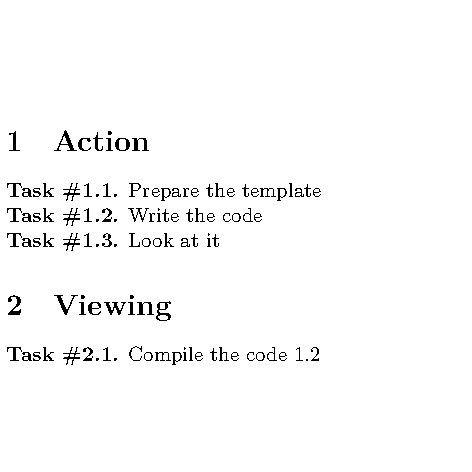
\includegraphics[width=\linewidth]{counterdom}
    \end{column}
    \inpause
    \begin{column}{0.45\textwidth}
    But the straightforward solution will give you 
    
    \vspace{-5ex}
    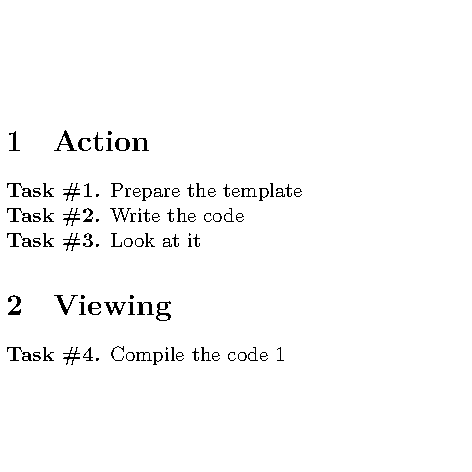
\includegraphics[width=\linewidth]{counterdomno}
         
    \end{column}
         
    \end{columns}
\end{frame}

\begin{frame}{Counter Domination\inclasshigh{\textit{(, conquering, humiliation)}}}{straightforward solution}\relax

    \twocolImg{
    % \lstinputlisting[linerange={11-20}]{counterdomno.tex}
    \inputminted[firstline=8, lastline=19]{latex}{sec/code/counters/counterdomno.tex}
    }{counterdomno}
    
    \inclassFrag{Try to compile it by your own}[0]
\end{frame}

\begin{frame}[fragile]{Counter Domination\inclasshigh{\textit{(, conquering, humiliation)}}}{The Way}\relax

    \newcommand{\modif}[3]{\fbox{\parbox{\textwidth}{\makebox[\textwidth]{\small\makebox[0.47\textwidth]{#1}\hfill$\to$\hfill\makebox[0.47\textwidth]{#2}}\\ #3}}}
    
    \centering
    \modif{\string\newcounter\{task\}}{\ocol\newcounter\{task\}[section]}{\ocol\newcounter\{<slave>\}[<master>] will resets the value of <slave> if the value of <master> is change}
    
    \inclassFrag{Please, modify your code after this and every step in this frame}
    % \inpause
    
    \modif{\ccol\addtocounter\{task\}\{1\}}{\ccol\refstepcounter\{task\}}{
    \ccol\refstepcounter\{<counter>\} use it to update \ccol\label--\ccol\ref\ mechanism
    }
    
    \inpause
    \modif{\string\textbf\{Task \string\#\string\arabic\{task\}.}{\tiny\string\textbf\{Task \string\#\string\arabic\{section\}.\string\arabic\{task\}.}{Inside \string\newcommand\{\string\tsk\} to redefine the labels}
    
    \inpause
    \modif{}{\tiny\string\renewcommand\{\ccol\thetask\}\{\string\arabic\{section\}.\string\arabic\{task\}\}}{\string\renewcommand\{\ccol{\the<counter>}\} to redefine the reference}
    
    \skfootnote{\lvoc{VII.3.3}[250] \lmanc{13.6}[128]}
\end{frame}

\begin{frame}{Counter Domination\inclasshigh{\textit{(, conquering, humiliation)}}}{solution}\relax
    \begin{columns}[t]
        \begin{column}{0.5\textwidth}
             \inputminted[firstline=8, lastline=19]{latex}{sec/code/counters/counterdomno.tex}
        \end{column}
        \begin{column}{0.6\textwidth}
             \inputminted[firstline=8, lastline=19]{latex}{sec/code/counters/counterdom.tex}
        \end{column}
         
    \end{columns}
     
\end{frame}

\begin{frame}{Counter Domination\inclasshigh{\textit{(, conquering, humiliation)}}}{solution}\relax
    \twocolImg{
    % \lstinputlisting[linerange={11-20}]{counterdom.tex}
    \inputminted[firstline=8, lastline=19]{latex}{sec/code/counters/counterdom.tex}
    }{counterdom}
\end{frame}



\begin{frame}[fragile]{Redefine existing counter domination\magicPage}{``equation'' example}\relax
    Package based solution:
    
    \lstinline|\usepackage{chngcntr}| 
    
    and \lstinline|\counterwith{equation}{chapter}|  to make the ``equation'' a slave or \lstinline|\counterwithout{equation}{chapter}| to ``free'' the counter.
    
    Core-based solution:

\begin{minted}{latex}
\makeatletter
\@removefromreset{equation}{section}
\@addtoreset{equation}{chapter}
\renewcommand{\theequation}{\thechapter.\@arabic\c@equation}
\makeatother
\end{minted}


    \skfootnote{\stExC{https://tex.stackexchange.com/questions/61756/how-to-change-equation-numbering-style} \stExC{https://tex.stackexchange.com/questions/54241/change-the-type-of-equation-numbering-in-document-class-article} \stExC{https://tex.stackexchange.com/questions/28333/continuous-v-per-chapter-section-numbering-of-figures-tables-and-other-docume} \normalfont\url{https://texfaq.org/FAQ-running-nos} \lvoc{IX.2.1}[293].\\ Also see \ccol{\p@} prefix \lvoc{IX.2.2}[295] and \stExC{https://tex.stackexchange.com/questions/61426/how-to-make-ref-display-only-subsection}}     
\end{frame}


\begin{frame}[fragile]{Define and simple manipulation\tW}\relax


     \textbf{Define new} \ccol\newcount\ccol{\<countname>} as \verb|\newcount\mycounter|
     
     \textbf{Set number} \ccol{\<countname>=<number>}  Or use \ccol\countdef. Like \verb|\countdef\mynumber=43|
     
     \textbf{Add number}  \ccol{\advance\string\<countname>\ by <number>}. Also there are \ccol\multiply\ and \ccol\divide. As well as \ccol\numexp.
     
     \textbf{Show number} \ccol{\the\string\<countname>} or \ccol\number\ or \ccol\romannumeral
     
     \skfootnote{\vspace{-3ex}\knuthc{15}[129] \stExC{https://tex.stackexchange.com/questions/245635/formal-syntax-rules-of-dimexpr-numexpr-glueexpr}\\Actually you can use \ccol\count<number> like \ccol\count212. What \ccol\newcount\ do is just find a free number and fix it to your defined name.}
\end{frame}

\begin{frame}{Define and simple manipulation\tW}{Example}\relax

    \twocolImg{
    % \lstinputlisting[linerange={11-16}]{counterTeX.tex}
        \inputminted[firstline=11, lastline=16]{latex}{sec/code/counters/counterTeX.tex}
    }{counterTeX}

\end{frame}

\graphicspath{{sec/images/}{sec/code/}}
\lstset{inputpath=sec/code/}

\subsection{Lengths}
% \knuthc  knuth the TeXBook
% \lvoc   Lvovsky
% \lamc  lamport latex 
% \slshape different font for footnote
\graphicspath{{sec03/images/s1/}{sec03/code/s1/}}
\lstset{inputpath=sec03/code/s1/}

\begin{frame}[fragile]{Going $\to$ Math}\relax

\cprotect\skfootnote{
\vspace{-0.5ex}
\lvoc{I.3.29}, \lamc{3.1}, \knuthc{16}[137] \\ {\slshape 
also try \verb|\(x=y\)| and \verb|\[x=y\]| and environment \verb|equation*|}\\
\textt \verb|\|lstinputlisting[firstline=7, lastline=14,linerange=\{8-10\}]\{file.tex\}
}

\cprotect\twocolImg{
Math environments

\lstinputlisting[linerange={15-16,19-19,22-25}]{mdollar.tex}
}{mdollar}

\end{frame}

\begin{frame}{Going $\to$ Math}\relax
{\centering \Large
``Because mathematics is supposedly expensive.''\par} 

\hfill \textcopyright D.~Knuth``the \TeX Book''
     \skfootnote{\knuthc{16}[138]}
\end{frame}


\begin{frame}[fragile]{Indexes}\relax

\newcommand{\appendTline}[3]{
\makebox[10em]{#1\hfill} \hfill\hfill \makebox[5em]{\hfill #2\hfill} \hfill \makebox[5em]{\hfill #3\hfill} \hfill\hfill \strut
    \hrule
    \vspace{1ex}
}

\cprotect[mm]\appendTline{upper ind}{\lstinline[basicstyle=\tt\normalsize,]|$x^2$|}{ $x^2$}

\cprotect[mm]\appendTline{lower ind}{\lstinline[basicstyle=\tt\normalsize,]|$x_2$|}{ $x_2$}
\cprotect[mm]\appendTline{lower and upper ind}{\lstinline[basicstyle=\tt\normalsize,]|$x^4_2$|}{ $x^4_2$}
\cprotect\inclassFrag{
Try to put more then one letter to the index}
\cprotect[mm]\appendTline{more letters in ind}{\lstinline[basicstyle=\tt\normalsize,]|$x_{ij}$|}{ $x_{ij}$}
\cprotect\inclassFrag{

How can you create ${}^3_2 He$?}[4]
\cprotect[mm]\appendTline{empty block}{\lstinline[basicstyle=\tt\normalsize,]|${}^3_2He$|}{ ${}^3_2He$}
\cprotect[mm]\appendTline{index in index}{\lstinline[basicstyle=\tt\normalsize,]|$x^{4^2}$|}{ $x^{4^2}$}

\skfootnote{\knuthc{16}[139]\\You really don't want to know, what code generate these lines...}
\end{frame}

\begin{frame}[fragile]{Fractions and (square) root}\relax
    \begin{columns}
        \begin{column}{0.45\textwidth}
          \hfill \lstinline[basicstyle=\tt\normalsize]|$\frac{x+z^2}{y-1}$| 
        \end{column}
        \begin{column}{0.45\textwidth}
             $$\frac{x+z^2}{y-1}$$
        \end{column}
    \end{columns}
    \vphantom.
    \hrule
    \vphantom) 
    \begin{columns}
        \begin{column}{0.45\textwidth}
          \hfill \lstinline[basicstyle=\tt\normalsize]|$\sqrt{x}$| 
        \end{column}
        \begin{column}{0.45\textwidth}
             $$\sqrt{x}$$
        \end{column}
    \end{columns}
    \vphantom(
    \hrule
    \vphantom) 
    \begin{columns}
        \begin{column}{0.45\textwidth}
          \hfill \lstinline[basicstyle=\tt\normalsize]|$\sqrt[y]{x}$| 
        \end{column}
        \begin{column}{0.45\textwidth}
             $$\sqrt[y]{x}$$
        \end{column}
    \end{columns}
    
\cprotect\skfootnote{\lmanc{16.7.3}[159] \lmanc{16.7.5}[160] \overC{https://www.overleaf.com/learn/latex/Fractions_and_Binomials} \slshape sometimes, if you want use fraction into fraction it is better to use \verb|\cfrac{x}{y}|. See typeography section or \lvoc{II.4.1, II.5.1}
also $\sphericalangle$ \verb|\genfrac|
}
\end{frame}

\begin{frame}[fragile]{Brackets\preMagicPage}\relax

You can't write just
\vphantom. 
    \begin{columns}
        \begin{column}{0.70\textwidth}
          \hfill \lstinline[basicstyle=\tt\normalsize]"$$(\frac{x}{y})$$" 
        \end{column}
        \begin{column}{0.3\textwidth}
             $$(\frac{x}{y})$$
        \end{column}
    \end{columns}
    \vphantom(
    \incPause
use \ccol{\left} and \ccol{\right}
     \vphantom. 
    \begin{columns}
        \begin{column}{0.70\textwidth}
          \hfill \lstinline[basicstyle=\tt\normalsize]"$$\left(\frac{x}{y}\right)$$" 
        \end{column}
        \begin{column}{0.3\textwidth}
             $$\left(\frac{x}{y}\right)$$
        \end{column}
    \end{columns}
    \vphantom(
    \incPause
or even like 
\vphantom. 
    \begin{columns}
        \begin{column}{0.70\textwidth}
          \hfill \lstinline[basicstyle=\tt\normalsize]"$$\left.\frac{x}{y}\right|_a^b$$" 
        \end{column}
        \begin{column}{0.3\textwidth}
             $$\left.\frac{x}{y}\right|_a^b$$
        \end{column}
    \end{columns}
    \vphantom(
\end{frame}

\begin{frame}[fragile]{Brackets\magicPage}\relax

Sometimes you need to manually set the bracket size. Then use something like this 
\vphantom. 
    \begin{columns}
        \begin{column}{0.70\textwidth}
          \hfill \lstinline[basicstyle=\tt\normalsize]"$$(\bigl( \Bigl( \biggl( \Biggl($$" 
        \end{column}
        \begin{column}{0.3\textwidth}
             $$(\bigl( \Bigl( \biggl( \Biggl($$
        \end{column}
    \end{columns}
    \vphantom(
    
    \vphantom. 
    \begin{columns}
        \begin{column}{0.70\textwidth}
          \hfill \lstinline[basicstyle=\tt\normalsize]"$$]\bigr] \Bigr] \biggr] \Biggr]$$" 
        \end{column}
        \begin{column}{0.3\textwidth}
             $$]\bigr] \Bigr] \biggr] \Biggr]$$
        \end{column}
    \end{columns}
    \vphantom(

\skfootnote{\knuthc{17}[147] \overC{https://www.overleaf.com/learn/latex/Brackets_and_Parentheses}}
     
\end{frame}

\inclassFrame{
\begin{frame}{Type these equations}{simple}\relax
\begin{equation}
     x^2-2y = h_{l_0^k}\tag{1}
\end{equation}
\begin{equation}
     \sqrt{h/(2a)}=t\tag{2}
\end{equation}

\begin{equation}
     \frac{x+y}{z_2 - \frac{1}{2}}=m\tag{3}
\end{equation}

\begin{equation}
     \left(\frac{x+y}{z}\right)=q\tag{4}
\end{equation}

\end{frame}
}

\inclassFrame{
\begin{frame}{Type these equations}{harder}\relax
\begin{equation}
    T_{N_1}(t) = \left.\frac{d}{dx_i} f^{\sqrt{n}}(z)\right/\left(\sqrt{\frac{m+e}{a}}-N\right) \tag{1}
\end{equation}

\end{frame}
}

\begin{frame}[fragile]{Text inside equations}\relax
Sometimes, you need to write a text \textit{inside} an equation

$$\frac{x+1}{y} = z; \hbox{if $x - 1 < y$, but not always!}$$

\cprotect\inclassFrag{try to type \lstinline[basicstyle=\tt]|$$\frac{x+1}{y} = z; if x - 1 < y, but not always!$$|}
but the direct solution remove all spaces! 
$$\frac{x+1}{y} = z; if x - 1 < y, but not always!$$
\incPause
Use \ccol{\hbox}:

\lstinline[basicstyle=\tt]|$$\frac{x+1}{y} = z; \hbox{if $x - 1 < y$, but not always!}$$| \incPause \hfill or~\ccol{\text}~from~{\csk amsmath}~package.  

\end{frame}

\inclassFrame{
\begin{frame}{g}\relax
     How will you type $g = 9.8 \frac{\hbox{m}}{\hbox{s}^2}$?
\end{frame}
}

\begin{frame}[fragile]{More symbols\preMagicPage}\relax
    \line{\hss\Large \url{http://detexify.kirelabs.org/classify.html}\hss}
    
    \inclassFrag{\centering
    Try to find the following symbols: \\ $\exists$,  $\to$, $\notin$, $\sim$, $\equiv$
    }[-1]
    
    \skfootnote{\vspace{-3ex}
    \wikiC{https://en.wikibooks.org/wiki/LaTeX/Special_Characters} \\
    \url{ftp://sunsite.icm.edu.pl/pub/CTAN/info/symbols/comprehensive/symbols-a4.pdf} (338 pages) \\ \url{https://www.rpi.edu/dept/arc/training/latex/LaTeX_symbols.pdf} (22 pages)}
\end{frame}

\begin{frame}[fragile]{More symbols\magicPage}{Greek letters}\relax
\footnotesize

\newlength{\myboxlen}%
\setlength{\myboxlen}{9em}

\newcommand{\showmsym}[1]{%
\makebox[\myboxlen]{\hfill\makebox[0.45\myboxlen]{\csk\hfill\string#1}\makebox[0.25\myboxlen]{$\to$}\makebox[0.3\myboxlen]{$#1$\hfill}\hfill}%
}
\showmsym{\alpha}\hfill
\showmsym{\beta}\hfill
\showmsym{\gamma}\hfill
\showmsym{\delta}\hfill
\showmsym{\epsilon}\hfill
\showmsym{\zeta}\hfill
\showmsym{\eta}\hfill
\showmsym{\iota}\hfill
\showmsym{\kappa}\hfill
\showmsym{\lambda}\hfill
\showmsym{\mu}\hfill
\showmsym{\nu}\hfill
\showmsym{\xi}\hfill
\showmsym{\tau}\hfill
\showmsym{\upsilon}\hfill
\showmsym{\rho}\hfill
\showmsym{\sigma}\hfill
\showmsym{\pi}\hfill
\showmsym{\phi}\hfill
\showmsym{\chi}\hfill
\showmsym{\psi}\hfill
\showmsym{\omega}\hfill
\makebox[\myboxlen]{}\hfill
\makebox[\myboxlen]{}\hfill
\makebox[\myboxlen]{}\hfill

\showmsym{\varepsilon}\hfill
\showmsym{\vartheta}\hfill
\showmsym{\varkappa}\hfill
\showmsym{\varrho}\hfill
\showmsym{\varphi}\hfill

~\\
\showmsym{\Gamma}\hfill
\showmsym{\Delta}\hfill
\showmsym{\Lambda}\hfill
\showmsym{\Xi}\hfill
\showmsym{\Sigma}\hfill
\showmsym{\Upsilon}\hfill
\showmsym{\Pi}\hfill
\showmsym{\Phi}\hfill
\showmsym{\Psi}\hfill
\showmsym{\Omega}\hfill
\makebox[\myboxlen]{}\hfill
\makebox[\myboxlen]{}\hfill
\makebox[\myboxlen]{}\hfill

\end{frame}

\begin{frame}[fragile]{More symbols\magicPage}{Other common used symbols}\relax
\footnotesize

\newlength{\myboxlen}%
\setlength{\myboxlen}{9em}

\newcommand{\showmsym}[1]{%
\makebox[\myboxlen]{\hfill\makebox[0.45\myboxlen]{\csk\hfill\string#1}\makebox[0.25\myboxlen]{$\to$}\makebox[0.3\myboxlen]{$#1$\hfill}\hfill}%
}
\showmsym{\infty}\hfill
\showmsym{\nabla}\hfill
\showmsym{\forall}\hfill
\showmsym{\partial}\hfill
\showmsym{\backslash}\hfill
\showmsym{\aleph}\hfill
\showmsym{\hbar}\hfill
\showmsym{\Re}\hfill
\showmsym{\Im}\hfill
\showmsym{\cdot}\hfill
\showmsym{\cdots}\hfill
\showmsym{\ldots}\hfill
\showmsym{\to}\hfill
\showmsym{\times}\hfill
\makebox[\myboxlen]{}\hfill
\makebox[\myboxlen]{}\hfill
\makebox[\myboxlen]{}\hfill

\normalsize
 \showmsym{\imath}\hfill \showmsym{\jmath}\hfill are useful for accents.

\end{frame}

\begin{frame}[fragile]{More symbols\magicPage}{Accents}\relax
% \footnotesize

\skfootnote{\knuthc{17}}
\newlength{\myboxlen}%
\setlength{\myboxlen}{9em}

\newcommand{\showmacc}[2]{%
\makebox[\myboxlen]{\hfill\makebox[0.45\myboxlen]{\hfill{\csk\string#1}\{#2\}}\makebox[0.25\myboxlen]{$\to$}\makebox[0.3\myboxlen]{$#1{#2}$\hfill}\hfill}%
}
\showmacc{\hat}{a}\hfill
\showmacc{\check}{a}\hfill
\showmacc{\tilde}{a}\hfill
\showmacc{\acute}{a}\hfill
\showmacc{\grave}{a}\hfill
\showmacc{\dot}{a}\hfill
\showmacc{\ddot}{a}\hfill
\showmacc{\breve}{a}\hfill
\showmacc{\vec}{a}\hfill
~\\[2ex]
\pause

\setlength{\myboxlen}{12em}
\Large \showmacc{\check}{a}\hfill \to \hfill
\setlength{\myboxlen}{13em}
{\csk \textbackslash{}skew5\textbackslash{}check}\{a\}{$\to$}$\skew5\check{a}$%

\end{frame}


\begin{frame}[fragile]{More symbols\magicPage}{Math fonts}\relax
    \begin{tabbing}
    ааaaaaaaaaaaaaaaaaaaaaaaaaaaaa \= aaaaaaaaaaaaaaaaaaaaaaaaaaaaaa \= \kill
    \texttt{\textbackslash mathrm\{\textit{letters,etc}\}} \> $\mathrm{ABCabc,123,\hat{a},\tilde{b},\tilde{c},\Psi\Omega}$ \\
    \texttt{\textbackslash mathbf\{\textit{letters,etc}\}} \> $\mathbf{ABCabc,123,\hat{a},\tilde{b},\tilde{c},\Psi\Omega}$ \\
    \texttt{\textbackslash mathsf\{\textit{letters,etc}\}} \> $\mathsf{ABCabc,123,\hat{a},\tilde{b},\tilde{c},\Psi\Omega}$ \\
    \texttt{\textbackslash mathtt\{\textit{letters,etc}\}} \> $\mathtt{ABCabc,123,\hat{a},\tilde{b},\tilde{c},\Psi\Omega}$ \\
    \texttt{\textbackslash mathit\{\textit{letters,etc}\}} \> $\mathit{ABCabc,123,\hat{a},\tilde{b},\tilde{c},\Psi\Omega}$ \\
    \texttt{\textbackslash mathnormal\{\textit{letters,etc}\}} \> $\mathnormal{ABCabc,123,\hat{a},\tilde{b},\tilde{c},\Psi\Omega}$ \\
    \texttt{\textbackslash mathcal\{\textit{capital letters}\}} \> $\mathcal{ABC}$ \\ 
    \texttt{\textbackslash mathds\{\textit{capital letters}\}} \> $\mathds{ABCRN}$ 
    \end{tabbing}
    \cprotect\skfootnote{\lstinline|\usepackage{dsfont}| for the last}
\end{frame}

\begin{frame}[fragile]{More symbols\magicPage}{Limiters}\relax
\skfootnote{\knuthc{17}}
\newlength{\myboxlen}%
\setlength{\myboxlen}{6em}
% \small
\newcommand{\showmsym}[1]{%
\makebox[\myboxlen]{\hfill\makebox[0.45\myboxlen]{\small\csk\hfill\string#1}\makebox[0.25\myboxlen]{$\to$}\makebox[0.3\myboxlen]{$$#1$$\hfill}\hfill}%
}
\newcommand{\showidenti}[1]{%
\makebox[\myboxlen]{\hfill\makebox[0.45\myboxlen]{\csk\hfill$#1$}\makebox[0.25\myboxlen]{$\to$}\makebox[0.3\myboxlen]{$$#1$$\hfill}\hfill}%
}
{\bfseries Brackets}

\showidenti{(}\hfill
\showidenti{)}\hfill
\showmsym{\langle}\hfill
\showmsym{\rangle}\hfill
\showidenti{[}\hfill
\showidenti{]}\hfill
\showmsym{\lbrack}\hfill
\showmsym{\rbrack}\hfill
\showmsym{\{}\hfill
\showmsym{\}}\hfill
\showmsym{\lbrace}\hfill
\showmsym{\rbrace}\hfill
\showmsym{\lfloor}\hfill
\showmsym{\rfloor}\hfill
\showmsym{\lceil}\hfill
\showmsym{\rceil}\hfill

{\bfseries Other}
\renewcommand{\to}{}

\showidenti{/}\hfill
\showmsym{\backslash}\hfill
\showidenti{|}\hfill
\showmsym{\vert}\hfill
\showmsym{\|}\hfill
\showmsym{\Vert}\hfill
\showmsym{\updownarrow}\hfill
\showmsym{\Updownarrow}\hfill
\showmsym{\uparrow}\hfill
\showmsym{\Uparrow}\hfill
\showmsym{\downarrow}\hfill
\showmsym{\Downarrow}\hfill

\end{frame}

\begin{frame}[fragile]{More symbols\magicPage}{Limiters with {\csk \string\Big} prefix}\relax
\skfootnote{\knuthc{17}[147]}
\newlength{\myboxlen}%
\setlength{\myboxlen}{6em}
% \small
\newcommand{\showmsym}[1]{%
\makebox[\myboxlen]{\hfill\makebox[0.45\myboxlen]{\scriptsize\csk\hfill\string#1}\makebox[0.25\myboxlen]{$\to$}\makebox[0.3\myboxlen]{$$\Big#1$$\hfill}\hfill}%
}


\showmsym{\vert}\hfill
\showmsym{\Vert}\hfill
\showmsym{\arrowvert}\hfill
\showmsym{\Arrowvert}\hfill
\showmsym{\lgroup}\hfill
\showmsym{\rgroup}\hfill
\showmsym{\lmoustache}\hfill
\showmsym{\rmoustache}\hfill
\showmsym{\bracevert}\hfill

\end{frame}

\begin{frame}[fragile]{More symbols\magicPage}{Operators}\relax
\skfootnote{\overC{https://www.overleaf.com/learn/latex/Integrals,_sums_and_limits}}

\newlength{\myboxlen}%
\setlength{\myboxlen}{9em}

\newcommand{\showmsym}[1]{%
\makebox[\myboxlen]{\hfill\makebox[0.45\myboxlen]{\csk\hfill\string#1}\makebox[0.25\myboxlen]{$\to$}\makebox[0.3\myboxlen]{$$#1$$\hfill}\hfill}%
}
\showmsym{\prod}\hfill
\showmsym{\sum}\hfill
\showmsym{\int}\hfill
\showmsym{\iint}\hfill
\showmsym{\oint}\hfill
\showmsym{\idotsint}\hfill

\end{frame}

\begin{frame}[fragile]{More symbols}{Operators}\relax
Mathematical tradition: write not $sin (x)$, but {\csk$\sin (x)$}.\incPause

\begin{center}
     \Large use \ccol{\sin}
\end{center}
\incPause
sometimes more effect is displayed:
\begin{columns}

\begin{column}{0.5\textwidth}
\hfill\lstinline[basicstyle=\tt]|$$\min_{x\to 0} f$$|     
\end{column}
\begin{column}{0.5\textwidth}
$$\min_{x\to 0} f$$
\end{column}
\end{columns}


    \skfootnote{\overC{https://www.overleaf.com/learn/latex/Operators} \knuthc{18}[173] \url{https://oeis.org/wiki/List_of_LaTeX_mathematical_symbols}}
\end{frame}

\begin{frame}[fragile]{Multiline equations\preMagicPage}\relax
     \cprotect\twocolImg{
        \lstinputlisting[linerange={9-14}]{arraySimple}
    }{arraySimple}

\incPause
notice {\csk \{clcl\}}, {\csk \&}, \ccol{\\}
\inclassFrag{Does it reminds you something?}[3]

\ccol{array} is a \ccol{tabular} for math mode!

\cprotect\skfootnote{{ } \lvoc{II.3}[75], \lvoc{II.4.2}[84] \lmanc{8.2}[55]}
\end{frame}

\begin{frame}[fragile]{Also array\magicPage}\relax
     \cprotect\twocolImg{
        \lstinputlisting[linerange={11-17}]{matrixesno}
    }{matrixesno}
    \cprotect\twocolImg{
    \lstinputlisting[linerange={9-16}]{equcaseno}
    }{equcaseno}

\cprotect\skfootnote{advanced: \knuthc{18}[186] \tugC{https://www.tug.org/utilities/plain/cseq.html\#vcenter-rp}}
\end{frame}

\begin{frame}[fragile]{Multiline equations\preMagicPage}\relax
 it is better to use 
 \begin{center}
 \Large \csk \verb|\usepackage{amsmath}|
 \end{center}
 
\cprotect\skfootnote{\normalfont \url{http://mirrors.mi.ras.ru/CTAN/macros/latex/required/amsmath/amsmath.pdf} \url{http://texdoc.net/texmf-dist/doc/latex/amsmath/amsldoc.pdf}}
\end{frame}


\begin{frame}[fragile]{Formula in multiple line\magicPage}\relax
\skfootnote{{ }\lvoc{II.4.2}[81]\\ You can modify the line gaps, push string to left or right,..}

    \cprotect\twocolImg{
\lstinputlisting[linerange={13-14, 17-20}]{multilines.tex}
}{multilines}

\end{frame}


\begin{frame}[fragile]{Multiple formulas\magicPage}\relax

% \vspace{-10ex}
    \cprotect\twocolImg{
\lstinputlisting[linerange={13-14, 17-21}]{gathermy.tex}
}{gathermy}

\incPause
% \vspace{-10ex}
notice \lstinline[basicstyle=\tt\normalsize]|\notag| !

\cprotect\skfootnote{{} \lvoc{II.4.2}[81]\\ \slshape  also see \verb'gather*' to ban numeration}

\end{frame}

\begin{frame}[fragile]{Multiple formulas and lines: alignment\magicPage}\relax
\cprotect\twocolImg{
    \lstinputlisting[linerange={13-14, 17-20}]{alignmy.tex}
}{alignmy}
\cprotect\twocolImg{
    \lstinputlisting[linerange={13-14, 17-22}]{splitmy}
}{splitmy}


ampersand {\csk \&} is stands for indent (as in tables)
\cprotect\skfootnote{{ }\lvoc{II.4.2}[82]\\  also see \verb'align*' to ban numeration}
\end{frame}

\begin{frame}[fragile, t]{Text inside equations\magicPage}\relax

\cprotect\twocolImg{
    \lstinputlisting[linerange={13-14, 17-23}]{alignetextwrong1.tex}
}{alignetextwrong1}

Problem:
\cprotect\twocolImg{
    \lstinputlisting[linerange={13-14, 17-23}]{alignetextwrong.tex}
}{alignetextwrong}

\end{frame}
\begin{frame}[fragile]{Text inside equations\magicPage}{solution}\relax
% \vspace{-1.3cm}
\cprotect\twocolImg{
    \lstinputlisting[linerange={13-14, 17-23}]{alignetext.tex}
}{alignetext}
\ccol{\text} and \ccol{\intertext}
% \inclassFrag{How will you type $g = 9.8 \frac{\text{m}}{\text{s}^2}$?}[-1]
\skfootnote{{} \lvoc{II.4.2}[83]}
\end{frame}

\begin{frame}[fragile]{System of equations\magicPage}\relax
% \vspace{-1.3cm}
\cprotect\twocolImg{
    \lstinputlisting[linerange={13-14, 17-24}]{equsis.tex}
}{equsis}
% \vspace{-2cm}
\cprotect\twocolImg{
    \lstinputlisting[linerange={13-14, 17-23}]{equcase}
}{equcase}
\skfootnote{{} \lvoc{II.4.2}[84]}
\end{frame}


\begin{frame}[fragile]{Matrix\magicPage}\relax
    \cprotect\twocolImg{
    \lstinputlisting[linerange={7-7, 11-18}]{matrixes}
}{matrixes}
\cprotect\skfootnote{{ } \lvoc{II.3}[74]\\ \slshape Also see \lstinline!matrix! without borders and \lstinline!vmpatrix! for |border|}
     
\end{frame}

\cprotect\inclassFrame{
\begin{frame}[fragile]{Try to type the following}\relax
\small
\verb!$$\sum_a^b x$$!, \hfill\verb!$$\sum\nolimits_a^b x$$!, \hfill\verb!$$\sum\limits_a^b x$$!

\verb!$\sum_a^b x$!, \hfill\verb!$\sum\nolimits_a^b x$!, \hfill\verb!$\sum\limits_a^b x$!

\verb!$$\int_a^b x$$!, \hfill\verb!$$\int\nolimits_a^b x$$!, \hfill\verb!$$\int\limits_a^b x$$!

\verb!$\int_a^b x$!, \hfill\verb!$\int\nolimits_a^b x$!, \hfill\verb!$\int\limits_a^b x$!
~\\[2ex]
compare the index position and the operator size
     
\end{frame}
}

\begin{frame}[fragile]{One over another\preMagicPage}{operators}\relax

\newcommand{\appendTline}[2]{\vspace*{10pt}\begin{columns}
        \begin{column}{0.45\textwidth}
          \hfill #1 
        \end{column}
        \begin{column}{0.45\textwidth}
             \hfill #2\hfill \hfill
        \end{column}
    \end{columns}
    \vphantom.
    \hrule
    }

    \cprotect[mm]\appendTline{\csk source}{\csk operator}
    \hrule height 0.05pt
    \cprotect[mm]\appendTline{\lstinline[basicstyle=\tt\normalsize,]|$$\int\limits_0^\pi$$|}{$$\int\limits_0^\pi$$}
    \cprotect[mm]\appendTline{\lstinline[basicstyle=\tt\normalsize,]|$$\int\nolimits_0^\pi$$|}{$$\int\nolimits_0^\pi$$}

\end{frame}

\begin{frame}[fragile]{One over another\magicPage}\relax

\newcommand{\appendTline}[2]{\vspace*{10pt}\begin{columns}
        \begin{column}{0.45\textwidth}
          \hfill #1 
        \end{column}
        \begin{column}{0.45\textwidth}
             \hfill #2\hfill \hfill
        \end{column}
    \end{columns}
    \vphantom.
    \hrule
    }

    \cprotect[mm]\appendTline{\csk source}{\csk result}
    \hrule height 0.05pt
    \cprotect[mm]\appendTline{\lstinline|$\stackrel {\Leftrightarrow}{A}$|}{$\stackrel {\Leftrightarrow}{A}$}
    \cprotect[mm]\appendTline{\lstinline|$A \stackrel{a'}{\rightarrow} D$|}{$A \stackrel{a'}{\rightarrow} D$}
    \cprotect[mm]\appendTline{\lstinline|$$\sum_{\substack{i\in[0;n]\\j\in[0;m]}} a_{ij}$$|}{$$\sum_{\substack{i\in[0;n]\\j\in[0;m]}} a_{ij}$$}
    
\end{frame}

\begin{frame}[fragile]{One over another\magicPage}\relax

\newcommand{\appendTline}[2]{\vspace*{10pt}\begin{columns}
        \begin{column}{0.45\textwidth}
          \hfill #1 
        \end{column}
        \begin{column}{0.45\textwidth}
             \hfill #2\hfill \hfill
        \end{column}
    \end{columns}
    \vphantom.
    \hrule
    }

    \cprotect[mm]\appendTline{\csk source}{\csk result}
    \hrule height 0.05pt
    
    \cprotect[mm]\appendTline{\lstinline|$\underbrace{a+\overbrace{b+c}+d}_{m}$|}{$\underbrace{a+\overbrace{b+c}+d}_{m}$}
    
    \cprotect[mm]\appendTline{\lstinline|$\lefteqn{\overbrace{ \phantom{1+2+3}}} 1+\underbrace{2+3+4}$|}{$\lefteqn{\overbrace{ \phantom{1+2+3}}} 1+\underbrace{2+3+4}$}
    
\end{frame}

\begin{frame}{Domain-specific packages}{Lots of them!}\relax
You can use 
    \begin{description}
        \item[Physics] \url{https://ctan.org/pkg/physics}
        \item[Chemistry] \url{http://www.mychemistry.eu/known-packages/}, \url{https://ru.overleaf.com/learn/latex/Chemistry_formulae}, \url{https://ctan.org/pkg/mhchem}
        \item[Biology] \url{https://www.tug.org/pracjourn/2007-4/senthil/senthil.pdf} 
    \end{description}
     
\end{frame}
\subsection{Boxes}
\graphicspath{{sec02/images/}{sec02/code/}}
\lstset{inputpath=sec02/code/}

\begin{frame}[label=style,fragile]{Built--in themes}
    \visible<1>{\hyperlink{simple}{\beamerbutton{SIMPLE}} \\}
    \lstinline[basicstyle=\tt]|\usetheme{CambridgeUS}|\\
    \lstinline[basicstyle=\tt]|\usecolortheme{crane}|\\
    \url{https://hartwork.org/beamer-theme-matrix/}\\ \pause
    \lstinline[basicstyle=\tt]|\usefonttheme{structureitalicserif}|\\
    \url{http://deic.uab.es/~iblanes/beamer_gallery/index_by_font.html}\\ 
    \vspace{1cm}
    \inclassFrag{Google \alert{Beamer Theme Matrix} and \alert{Beamer font theme gallery}.}[-1]
\end{frame}

\cprotect\inclassFrame{
\begin{frame}[fragile]{Compile your beamer presentation}\relax
    \only<1>{ \lstinputlisting[basicstyle=\tt\footnotesize, numbers=none]{task1.tex} }
    \only<2>{ \lstinputlisting[basicstyle=\tt\footnotesize, numbers=none]{task2.tex} }
    \only<3>{ \lstinputlisting[basicstyle=\tt\footnotesize, numbers=none]{task3.tex} }
\end{frame}
}

\begin{frame}[fragile]{Colors}
    \skfootnote{\url{en.wikibooks.org/wiki/LaTeX/Colors}}
    \LaTeX provides several standart colors: 
    \textcolor{red}{red}, \textcolor{blue}{blue}, \textcolor{green}{green},\dots\\
    \lstinline[basicstyle=\tt]|\textcolor{red}{text}| \\
    \pause
    There many ways to define new colors, e.~g.
    \lstinline[basicstyle=\tt]|\definecolor{orange}{rgb}{1,.5,0}|\\
    \lstinline[basicstyle=\tt]|\definecolor{orange}{RGB}{255,127,0}|
\end{frame}

\begin{frame}{Colors}
    Beamer automatically loads \alert{xcolor} package\\
    Somehow popular way to define new colors is buy the following rule
    \begin{table}
    \begin{tabular}{0.7\textwidth}\hline
        color           &   rgb formula             &     output  \\\hline
        red!30!blue     &   .3(1,0,0)+.7(0,0,1)     &   \textcolor{red!30!blue}{example} \\
        red!30          &   .3(1,0,0)+.7(1,1,1)     &   \textcolor{red!30!}{example}    \\ 
        red!30!blue!50!green    &   .5(red!30!blue)+.5(0,1,0)   &   \textcolor{red!30!blue!50!green}{example}   
    \end{tabular}          
    \end{table}
\end{frame}

\begin{frame}[t,fragile]{Customazation}
        \lstinline[basicstyle=\tt]|\begin{block}{Block title}|  \\
        \lstinline[basicstyle=\tt]|     Block body|  \\
        \lstinline[basicstyle=\tt]|\end{block}| \\
\end{frame}

\begin{frame}[t,fragile]{Customazation}
        \begin{block}{Block title}
            Block body
        \end{block}
    \pause\vspace{5mm}
    \lstinline[basicstyle=\tt]|\setbeamercolor{block title}{bg=blue!90,fg=white}|
    \lstinline[basicstyle=\tt]|\setbeamercolor{block body}{bg=blue!40!,fg=black}|
    \lstinline[basicstyle=\tt]|\setbeamertemplate{blocks}[rounded][shadow=true]|
    \setbeamercolor{block title}{bg=blue!90,fg=white}
    \setbeamercolor{block body}{bg=blue!40!,fg=black}
    \setbeamertemplate{blocks}[rounded][shadow=true]
    \pause
    \begin{block}{Block title}
          Block body
    \end{block}
\end{frame}

\begin{frame}[fragile]{beamerskoltech.sty}
\skfootnote{github.com/lavton/SkoltechLaTeXtemplates}
    This presentation uses package \\
    \lstinline[basicstyle=\tt]|\usepackage[logo]{beamerskoltech}|\\
    \pause
    This package manages styling and allows to use commands like \
    \lstinline[basicstyle=\tt]|\skfootnote{github.com/lavton/SkoltechLaTeXtemplates}|\\
    \inclassFrag{Upload \texttt{beamerskolthech.sty} from Canvas and compile document with it }[-1]
\end{frame}


\subsection{Glue}
% \knuthc  knuth the TeXBook
% \lvoc   Lvovsky
% \lamc  lamport latex 
% \slshape different font for footnote
\graphicspath{{sec01/images/s3/}{sec01/code/s3/}}
\lstset{inputpath=sec01/code/s3/}

\begin{frame}[fragile]{\ccol{\footnote}\magicPage}\relax
\cprotect\twocolImg{
    \lstinputlisting[linerange={9-9}]{footnoteMy.tex}
}{footnoteMy}  


\skfootnote{\lmanc{8}[108] \wikiC{https://en.wikibooks.org/wiki/LaTeX/Footnotes_and_Margin_Notes} \overC{https://www.overleaf.com/learn/latex/Footnotes} \knuthc{15}[120]}
\end{frame}

\begin{frame}[fragile]{Horizontal aligment\magicPage}\relax
\cprotect\twocolImg{
    \lstinputlisting[linerange={9-25}]{flushing.tex}
}{flushing}  


\skfootnote{\lmanc{8.12}[63] \lmanc{8.13}[64] \knuthc{14}[112] and note \stExC{https://tex.stackexchange.com/questions/64644/centering-doesnt-seem-to-center-my-text}}
\end{frame}

\begin{frame}[fragile]{Page break\magicPage}\relax

{\centering \Large \ccol{\newpage} \ccol{\pagebreak}\par}

\skfootnote{\lmanc{10}[105] \stExC{https://tex.stackexchange.com/questions/736/pagebreak-vs-newpage}}
     
\end{frame}

\begin{frame}[fragile]{Quotes\magicPage}\relax

\cprotect\twocolImg{
    \lstinputlisting[linerange={10-14}]{quotemy.tex}
}{quotemy}  


\cprotect\skfootnote{\lvoc{III.7.1}[129] \lmanc{8.20}[83]. Also see \verb|quotation| env }
     
\end{frame}

\begin{frame}[fragile]{Verses\magicPage}\relax

\cprotect\twocolImg{
    \lstinputlisting[linerange={11-18}]{versemy.tex}
}{versemy}  

\skfootnote{\lvoc{III.7.3}[130] \lmanc{8.28}[98]}
\end{frame}

\begin{frame}[fragile]{Marginal notes\magicPage}\relax

\cprotect\twocolImg{
    \lstinputlisting[linerange={9-10}]{marginmy.tex}
}{marginmy}  

\skfootnote{\lvoc{IV.10}[194] \lmanc{15.4}[137]}
\end{frame}

 
\cprotect\inclassFrame{
\begin{frame}[fragile]{Try to add a package}\relax
\url{http://hanno-rein.de/downloads/coffee.sty}

and use \verb|\newpage \coffee{2} hello world!|

\incPause
NOW you document is ready!

\end{frame}
}
\subsection{Spaces}
\graphicspath{{sec03/images/}{sec03/code/}}
\lstset{inputpath=sec03/code/}

% phantom, smash
\begin{frame}{What spaces we have?}
     \def\showLength#1{\newbox\boxtodimen%
\newdimen\wb%
\setbox\boxtodimen=\hbox{#1}%
\wb=\the\wd\boxtodimen%
     \leavevmode\raise4pt\hbox{\vrule height 6pt depth2pt{\csk\rule{\wb}{4pt}}\vrule height 6pt depth2pt}%
     }
     
    \begin{columns}
    \begin{column}{0.45\textwidth}
    
\centering\Large
     \begin{tabular}{rl}
          \ccol\qquad& \showLength{\qquad}\\ 
          \ccol\quad& \showLength{\quad}\\ 
          \ccol\enspace & \showLength\enspace\\
          \ccol\  & \showLength{\ }\\
     \end{tabular}
     
     \ccol\quad\ is used below:
     $$x=y\quad\hbox{if y=0}$$
    \end{column}
    \begin{column}{0.45\textwidth}
    
\centering\Large
     \begin{tabular}{rl}
          \multicolumn{2}{c}{useful for math:}\\
          \ccol{\;} & \showLength{\;}\\
          \ccol{\>} & \showLength{$\>$}\\
          \ccol{\,} & \showLength{\,}\\
          \ccol{\!} & \showLength{\!}\\
     \end{tabular}
     
     the last one is negative space
    \end{column}
    \end{columns}
     
     
     \skfootnote{\knuthc{18}[178] \lmanc{19.1}[167]}
\end{frame}

\begin{frame}{Phantoms}\relax

Phantoms have the same size as it's an argument without drawing.\incPause 

\twocolImg{
\lstinputlisting[linerange={39-45}]{phantomsmy.tex}
}{phantomsmy}
\ccol\phantom\ leaves both dimentions. \ccol\hphantom\ and \ccol\vphantom\ leaves only one dimention.

\ccol\strut\ is short for \ccol\vphantom\{(\}

\ccol\smash\ is using to leave only the horizontal coordinate of a formula

\skfootnote{\lmanc{16.6}[156] \knuthc{18}[178]}
     
\end{frame}
\subsection{Toks}
\begin{frame}{Toks manipulation\tW\magicPage}\relax
    \TeX\ has addition registers for storing strings. They have \ccol\toks\ prefix/suffix. The difference between toks and storage inside macros are in extension (We mention the extension mechanism at the last lecture). In toks \TeX store tokens (unexpanded).
     
     \skfootnote{\stExC{https://tex.stackexchange.com/questions/455208/token-register-vs-macro-register}}
\end{frame}
\subsection{Inserts}
\begin{frame}{Inserts\tW\magicPage}\relax

    \TeX\ has addition registers for storing floats. They have \ccol\insert\ prefix/suffix. 
     
     \skfootnote{\knuthc{15}[132] \stExC{https://tex.stackexchange.com/questions/527613/simple-example-of-using-newinsert-and-friends}\\ But I failed to make a working example...}
\end{frame}


\inclassframe{

\begin{frame}{\exFrame{Make footnote center}}{lvl 1}\relax
    Update the code of footnote generation from previous exercise and make the following change:
    \begin{itemize}
        \item Make a spaces between frame number, footnote an year (see next frame)
        \item Please, use only glue commands
         
    \end{itemize}
\end{frame}

\begin{frame}[t]{\exFrame{Implement footnotes}}{lvl 1}\relax
    \centering
    \vspace*{-1cm}
    \fbox{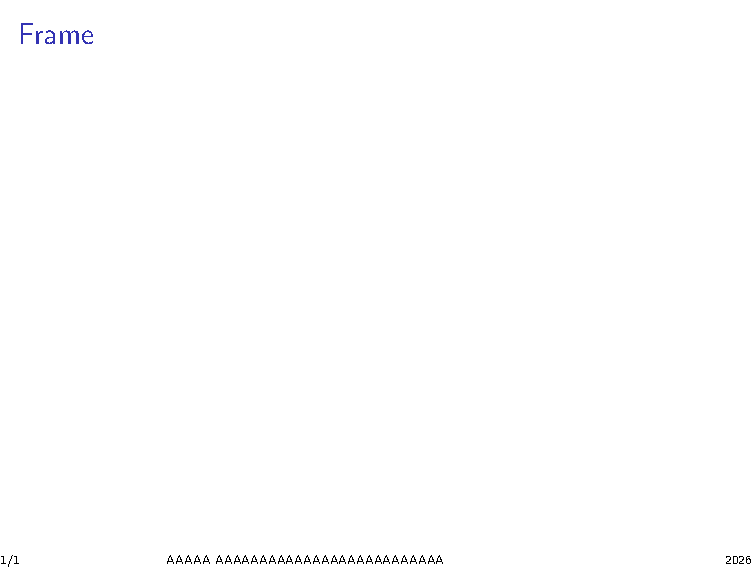
\includegraphics[scale=0.8]{exLvl1.pdf}}
\end{frame}

\begin{frame}{\exFrame{Make footnote center}}{lvl 2}\relax
     Update the previous template. 
     \begin{itemize}
         \item Remove year information from the right
         \item Make the footnote appears \textit{exactly} at the center independing of how width are slide number infrormation
         \item Check one and multiline footnote 
         \item You can use all build-in possibilities
     \end{itemize}
\end{frame}

}



\progressend


\begin{frame}\frametitle{What we have learned today?}\relax
    \tableofcontents
\end{frame}

\begin{frame}[allowframebreaks]{references}
color from the footnotes corresponds to references' color.
    \begin{itemize}
        \item \knuthc{Knuth ``The \TeX Book''}
        \item \lvoc{L'vovsky ``Nabor i verstka v sisteme \LaTeX''}
        \item \lamc{Lamport. ``\LaTeX. A Document Preparation System, User’s Guide and Reference Manual''}
        \item \lmanc{``\LaTeX 2e: An unofficial reference manual''} also at website \url{https://latexref.xyz/}
        \item \stExC{https://tex.stackexchange.com/questions} : \url{https://tex.stackexchange.com/questions}
        \item \wikiC{https://en.wikibooks.org/wiki/LaTeX} : \url{https://en.wikibooks.org/wiki/LaTeX}
        \item \overC{https://www.overleaf.com/learn/latex} : \url{https://www.overleaf.com/learn/latex}
        \item \tugC{https://www.tug.org/utilities/plain/cseq.html} : \url{https://www.tug.org/utilities/plain/cseq.html}
    \end{itemize}
\end{frame}

\begin{frame}{Distribution}\relax
\begin{itemize}
     \item the pdf-version of the presentation and all printed materials can be distributed under license Creative Commons Attribution-ShareAlike 4.0 \url{https://creativecommons.org/licenses/by-sa/4.0/}
     \item The source code of the presentation is available on {\csk\url{https://github.com/Lavton/latexLectures}} and can be distributed under the MIT license \url{https://en.wikipedia.org/wiki/MIT_License\#License_terms}
\end{itemize}
     
\end{frame}
\end{document}